\documentclass[12pt]{article}
\usepackage{graphicx}
\usepackage{booktabs}
\usepackage{hyperref}
\usepackage{natbib}
\usepackage{multirow}
\usepackage{float}
\usepackage{placeins}

\graphicspath{ {./images/} }

% Force floats to stay within their section
\let\oldsection\section
\renewcommand{\section}[1]{\FloatBarrier\oldsection{#1}}


\title{Benchmarking Hyperparameter Optimization Strategies for Graph Neural Networks on ADMET Prediction Under Scaffold-Split Evaluation}
\author{
  Martin Stamenov$^{1,*}$, Mila Gjurovska$^{1}$,
  Viktorija Vodilovska$^{1}$, Ilinka Ivanoska$^{1}$ \\[6pt]
  \small $^{1}$[Department, University/Institution, City, Country] \\
  \small $^{*}$Corresponding author: [email@example.com]
}
\date{}

\begin{document}
\maketitle

\begin{abstract}
Hyperparameter optimization (HPO) is critical for Graph Neural Network (GNN) performance on molecular property prediction, yet systematic comparisons of HPO strategies under realistic evaluation protocols remain scarce. We benchmark seven HPO algorithms---Random Search, Particle Swarm Optimization (PSO), Artificial Bee Colony (ABC), Genetic Algorithm (GA), Simulated Annealing (SA), Hill Climbing (HC), and Tree-structured Parzen Estimator (TPE)---for GNN-based ADMET prediction across six Therapeutics Data Commons tasks under scaffold-split evaluation. Over 2{,}100 training runs, we find that \emph{no optimizer consistently dominates across tasks}: Random Search wins three of four regression tasks, while SA and ABC lead on toxicity classification. Crucially, no metaheuristic achieves a statistically significant improvement over Random Search under a 50-trial budget (Wilcoxon signed-rank, $p > 0.05$), indicating that scaffold-split evaluation erodes the advantages of adaptive search by introducing a noisier validation landscape. We further show that HPO-optimized task-specific GNNs match or exceed frozen pretrained encoders (ChemBERTa, MolCLR, Morgan fingerprints) on five of six tasks. Multi-seed validation confirms result robustness. These findings caution against generalizing HPO recommendations from random-split experiments and offer practical guidance for strategy selection under limited compute budgets.
\end{abstract}

\paragraph*{Keywords:} graph neural networks, hyperparameter optimization, ADMET prediction, scaffold-split, benchmarking, metaheuristic optimization, drug discovery

\section{Introduction}

Predicting molecular ADMET (Absorption, Distribution, Metabolism, Excretion, and Toxicity) properties is a central task in computational drug discovery, enabling early identification of promising candidates and flagging safety liabilities before costly synthesis and \emph{in vivo} testing~\cite{zhang2025admet}. Graph Neural Networks (GNNs) have emerged as a leading approach for this task: by operating directly on molecular graphs---atoms as nodes, bonds as edges---they learn task-specific representations through message passing, capturing both local functional groups and longer-range topological motifs that fixed-length fingerprints miss~\cite{gilmer2017neural, yang2019analyzing, xiong2020pushing}.

However, GNN performance is highly sensitive to hyperparameter configuration, and the choice of hyperparameter optimization (HPO) strategy interacts with the evaluation protocol in ways that are poorly understood. Under random data splits, sophisticated optimizers (Bayesian, evolutionary) often outperform simple baselines, but random-splits inflate performance estimates by allowing structurally similar molecules to appear in both training and test sets. Scaffold-based splitting~\cite{doi:10.1021/jm9602928}, which partitions compounds by Bemis--Murcko core structures, creates a more realistic generalization setting that mirrors prospective drug discovery campaigns. Under scaffold-splits, the validation landscape becomes noisier, potentially eroding the advantage of adaptive HPO methods~\cite{wu2018moleculenet, yang2019analyzing}. Despite this, systematic HPO comparisons under scaffold-split evaluation remain scarce in the molecular ML literature.

We address this gap by benchmarking seven HPO strategies---Random Search, Particle Swarm Optimization (PSO), Artificial Bee Colony (ABC), Genetic Algorithm (GA), Simulated Annealing (SA), Hill Climbing (HC), and Tree-structured Parzen Estimator (TPE)---for GNN-based ADMET prediction across six tasks from the Therapeutics Data Commons (TDC)~\cite{huang2021therapeuticsdatacommonsmachine}. The TDC provides standardized datasets with scaffold-based splits and public leaderboards, enabling fair comparison. Our experimental design encompasses 2{,}100+ model training runs (50 trials $\times$ 7 algorithms $\times$ 6 datasets), multi-seed validation, and statistical significance testing. As an additional reference, we compare optimized GNNs against pretrained molecular encoders (ChemBERTa, MolCLR, Morgan fingerprints) used as frozen feature extractors.

Unlike prior work proposing new molecular architectures, our focus is on \emph{evaluation methodology}: understanding how the choice of HPO strategy and splitting protocol interact to determine reported model performance.

\paragraph{Contributions.}
\begin{itemize}
    \item \textbf{Systematic HPO benchmark under scaffold-split.} We present the first large-scale empirical comparison of seven HPO algorithms for GNN-based ADMET prediction under scaffold-split evaluation, encompassing 2{,}100+ training runs with multi-seed validation and Wilcoxon significance tests. We demonstrate that no metaheuristic achieves a statistically significant improvement over Random Search at a 50-trial budget ($p > 0.05$), directly challenging optimizer recommendations derived from random-split experiments.
    \item \textbf{Evidence that evaluation protocol shapes optimizer conclusions.} We show that scaffold-based splitting alters HPO algorithm rankings compared to random-split settings, with Random Search leading on regression and SA/ABC on classification. This task- and protocol-dependence demonstrates that HPO benchmarking conclusions are not transferable across evaluation protocols---a methodological finding with implications beyond our specific experiments.
    \item \textbf{Practical HPO selection guidance.} We derive actionable recommendations for HPO strategy selection based on task type, compute budget, and dataset characteristics, and show that HPO-optimized task-specific GNNs match or exceed frozen pretrained encoders on five of six ADMET tasks.
\end{itemize}

\section{Related Work}

\subsection{ADMET Prediction}

The TDC ADMET benchmark~\cite{huang2021therapeuticsdatacommonsmachine} has become the standard evaluation platform for molecular property prediction. Table~\ref{tab:related_work_summary} summarizes representative approaches from the TDC leaderboard and the broader literature.

\begin{table}[htbp]
\centering
\caption{Summary of representative molecular property prediction methods. Performance is reported for selected TDC ADMET tasks under scaffold-split where available. GNN = Graph Neural Network, FP = Fingerprint, TF = Transformer.}
\label{tab:related_work_summary}
\scriptsize
\begin{tabular}{llp{4.2cm}l}
\toprule
\textbf{Method} & \textbf{Type} & \textbf{Key Approach} & \textbf{Ref.} \\
\midrule
\multicolumn{4}{l}{\emph{Traditional / Ensemble Methods}} \\
\midrule
MapLight & FP+ML & Morgan FP with RF and SVM on node embeddings & \cite{maplight} \\
FCA & Ensemble & Weighted combination of RF, XGBoost, and SVM & \cite{cfa} \\
RDKit2D + MLP & FP+ML & 200 physicochemical descriptors with MLP & \cite{rdkit2d_mlp} \\
\midrule
\multicolumn{4}{l}{\emph{Graph Neural Networks}} \\
\midrule
AttentiveFP & GNN & GCN/GAT layers with GRU-based attention readout & \cite{attentiveFP} \\
GCN & GNN & Multi-layer graph convolution with mean pooling & \cite{kipf2017gcn} \\
GIN & GNN & Graph isomorphism layers for WL-test expressivity & \cite{xu2019gin} \\
D-MPNN & GNN & Directed message passing on bonds & \cite{yang2019dmpnn} \\
MPNN++ & GNN & Enhanced message passing ($\sim$10M params) & \cite{miniMol} \\
\midrule
\multicolumn{4}{l}{\emph{Self-Supervised / Pretraining}} \\
\midrule
Attr.\ Masking & GNN+SSL & Node/edge attribute masking for pretraining & \cite{attrMasking} \\
GraphCL & GNN+SSL & Graph-level contrastive learning with augmentations & \cite{contrativeLearning} \\
MolCLR & GNN+SSL & Molecular contrastive learning of representations & \cite{molclr} \\
\midrule
\multicolumn{4}{l}{\emph{Foundation Models}} \\
\midrule
ChemBERTa-2 & TF & RoBERTa pretrained on 77M SMILES (ZINC) & \cite{chemberta2} \\
MolBERT & TF & BERT with SMILES and physicochemical objectives & \cite{molbert} \\
MolE & GNN+FM & Multi-task pretrained GNN encoder & \cite{molE} \\
DeepMol & GNN+FM & Deep molecular representation learning & \cite{deepMol} \\
MegaMolBART & TF & BART-based molecular generation and encoding & \cite{mmelon} \\
MiniMol & GNN+FM & Compact foundation model using MPNN++ & \cite{miniMol} \\
\bottomrule
\end{tabular}
\end{table}

The TDC leaderboards reveal that several top-performing approaches rely on comparatively simple architectures. MapLight~\cite{maplight} uses random forests and SVMs on node embeddings, while RDKit2D+MLP~\cite{rdkit2d_mlp} passes 200 physicochemical descriptors through a standard multi-layer perceptron. On certain datasets, even Random Forest or XGBoost achieves top results, motivating ensemble approaches such as FCA~\cite{cfa}, which combines multiple classifiers via weighted voting.

Among GNN-based methods, AttentiveFP~\cite{attentiveFP} employs GCN/GAT layers with GRU-based attention readout, achieving top-5 results on many TDC datasets. Standard architectures appearing prominently in molecular benchmarks include GCN~\cite{kipf2017gcn}, GIN~\cite{xu2019gin}, and D-MPNN~\cite{yang2019dmpnn}, which operates on bond-level rather than atom-level messages.

Self-supervised pretraining has been adapted from NLP to molecular graphs via two main paradigms: attribute masking~\cite{attrMasking}, which reconstructs removed node or edge features, and contrastive learning~\cite{contrativeLearning}, which trains encoders to produce similar embeddings for augmented views of the same molecule. MolCLR~\cite{molclr} extends contrastive learning with three graph augmentation strategies (atom masking, bond deletion, subgraph removal), demonstrating improved downstream ADMET prediction compared to training from scratch.

These techniques underpin most molecular foundation models, which follow a common paradigm: self-supervised pretraining on large unlabeled corpora, optional multi-task supervised training, and task-specific fine-tuning. Representative examples include DeepMol~\cite{deepMol}, MolE~\cite{molE}, and MegaMolBART~\cite{mmelon}. ChemBERTa~\cite{chemberta2} takes a distinct approach, applying a RoBERTa transformer to SMILES strings pretrained on 77M molecules from ZINC-15, while MolBERT~\cite{molbert} combines SMILES masked language modeling with auxiliary physicochemical objectives. A practical concern with foundation models is their large parameter count; MiniMol~\cite{miniMol} addresses this by using MPNN++ ($\sim$10M parameters) to achieve competitive TDC performance at substantially lower computational cost.

\paragraph{Scaffold Split Challenges.}
Transformer-based models can exhibit substantial scaffold-split degradation, achieving high validation AUC but near-random test performance~\cite{yang2019dmpnn,chemberta2}. Wu et al.~\cite{wu2018moleculenet} introduced MoleculeNet with scaffold-splitting to more faithfully reflect prospective drug discovery generalization. Our experiments confirm this: on Tox21 NR-AR, ChemBERTa achieves validation AUC~=~0.896 but drops to 0.73 on the scaffold-split test set, while MolCLR degrades to 0.54 (near random).


\subsection{Hyperparameter Optimization for Molecular ML}

HPO is a key performance driver in molecular ML, where small, noisy datasets amplify sensitivity to hyperparameter configuration. Bergstra and Bengio~\cite{bergstra2012random} established Random Search as a strong baseline, showing it outperforms grid search when only a subset of hyperparameters is influential. Bayesian methods such as TPE~\cite{bergstra2011tpe}, implemented in Optuna~\cite{akiba2019optuna}, improve sample efficiency by modeling the hyperparameter--performance relationship, making them attractive under limited trial budgets.

Population-based metaheuristics---PSO~\cite{kennedy1995pso}, GA~\cite{holland1975ga}, ABC~\cite{karaboga2005abc}---provide broader exploration but may require larger budgets to converge. SA~\cite{saopt} offers a middle ground by accepting suboptimal moves early to escape local optima. Despite widespread use in combinatorial optimization, systematic comparisons of these HPO strategies for molecular property prediction remain scarce, particularly under scaffold-split protocols. Our work addresses this gap.


\subsection{Challenges in Molecular ML: Distribution Shifts and Generalization}
Beyond the scaffold-split sensitivity discussed above, molecular property prediction faces additional generalization challenges that compound evaluation difficulty. First, ADMET datasets are typically small (hundreds to low thousands of compounds), which amplifies variance across data splits and makes HPO-selected configurations sensitive to the specific training fold~\cite{wu2018moleculenet}. Second, the relationship between molecular structure and pharmacokinetic endpoints is often indirect: properties such as clearance and half-life depend on enzyme kinetics, transporter activity, and protein binding factors not explicitly encoded in molecular graphs or SMILES strings~\cite{obach1999prediction}. Third, class imbalance in toxicity assays (e.g., 3.5\% positive rate in Tox21 NR-AR) biases standard loss functions toward the majority class, a problem that persists in our experiments where no explicit class reweighting is applied (see Section~\ref{sec:discussion}).

These compounding factors mean that reported model rankings can shift substantially depending on dataset size, splitting protocol, and evaluation metric. Robust benchmarking therefore requires multi-seed validation, significance testing, and confidence intervals---practices that remain inconsistent in molecular ML. Our framework enforces all three across every comparison.


\section{Materials and methods}

\subsection{Datasets and Evaluation Protocol}
\label{sec:datasets}

We evaluate all models on six molecular property prediction tasks drawn from the
Therapeutics Data Commons (TDC) ADMET benchmark~\cite{huang2021therapeuticsdatacommonsmachine},
covering four pharmacokinetic (ADME) regression tasks and two toxicity classification
tasks.  Figure~\ref{fig:class-distribution} provides an overview of data provenance
and class composition across all six datasets, highlighting the severe class
imbalance present in the toxicity benchmarks.

\subsubsection*{ADME Regression Tasks}

\paragraph{Caco-2 Permeability (Caco2\_Wang).}
The Caco-2 cell monolayer assay is the gold-standard \emph{in vitro} surrogate for
human intestinal absorption~\cite{artursson1991caco2}.  High apparent permeability
($P_{app} > 10^{-6}$ cm/s) is associated with good oral bioavailability.  The
dataset, curated by Wang et al.~\cite{wang2016admet}, contains \textbf{910 compounds}
with target values already expressed in log(cm/s) units; no further log transformation
is applied.  Caco-2 is considered the most tractable regression task in our benchmark
because permeability is governed primarily by molecular size, lipophilicity, and
hydrogen-bond capacity, features that GNNs can capture directly from atom graphs.

\paragraph{Half-Life Prediction (Half\_Life\_Obach).}
Plasma half-life ($t_{1/2}$, hours) determines dosing frequency and is essential for
designing drugs with adequate therapeutic windows.  However, half-life is a composite
pharmacokinetic parameter influenced not only by molecular structure but also by
volume of distribution, protein binding fraction, and individual patient
variability~\cite{obach1999prediction}.  The dataset is drawn from the Obach
FDA-approved drug collection and contains \textbf{667 compounds}
spanning a wide dynamic range (0.5-100$+$ hours).  We apply a log transformation
before standardization to reduce target skewness.

\paragraph{Hepatocyte Clearance (Clearance\_Hepatocyte\_AZ).}
Intrinsic clearance measured in freshly isolated human hepatocytes
($\mu$L/min/10$^6$ cells) captures both phase-I and phase-II metabolic routes and
is the most physiologically relevant \emph{in vitro} metabolic stability
assay~\cite{riley2001pharma}.  The dataset was generated internally at AstraZeneca
and is distributed through TDC~\cite{huang2021therapeuticsdatacommonsmachine},
comprising \textbf{1\,213 proprietary compounds}.
Low clearance values indicate slow hepatic elimination and a longer \emph{in vivo}
half-life.  This task proved the most challenging in our benchmark, with GNN models
yielding negative R$^2$ values, indicating that molecular structure alone is
insufficient to explain the variance in hepatic metabolism (see
Section~\ref{results}).

\paragraph{Microsomal Clearance (Clearance\_Microsome\_AZ).}
Human liver microsomal assays ($\mu$L/min/mg protein) measure primarily cytochrome
P450-mediated (CYP) oxidative metabolism; they offer higher throughput than
hepatocyte assays but capture only phase-I reactions~\cite{obach2006trend}.  The
AstraZeneca dataset contains \textbf{1\,102 compounds}.
Like hepatocyte clearance, microsomal clearance values are log-transformed and
then standardized using train-set statistics.

\subsubsection*{Toxicity Classification Tasks}

\paragraph{Tox21 Nuclear Receptor: Androgen Receptor (Tox21 NR-AR).}
The Tox21 initiative~\cite{tox21data} assembled a large multi-assay toxicology
panel spanning nuclear receptor signaling and stress response pathways to enable
high-throughput environmental hazard screening.  We use the \textbf{NR-AR} assay
(androgen receptor agonism), which identifies compounds that can disrupt androgen
signaling, a key mechanism in endocrine disruption and reproductive
toxicity.  The TDC catalogue lists
\textbf{7\,258 compounds} (6\,533 after graph conversion), of which only $\approx3.5\%$ are active (positive) samples
(see Figure~\ref{fig:class-distribution}), making this the most class-imbalanced
task in our benchmark.  Classification models are trained with standard binary
cross-entropy loss with logits; no explicit class reweighting is applied, which
may limit minority-class recall (see Section~\ref{sec:discussion}).

\paragraph{hERG Cardiotoxicity (hERG).}
Blockade of the hERG potassium ion channel is the predominant mechanism of
drug-induced QT interval prolongation and potentially fatal cardiac arrhythmias,
and the hERG assay is a mandatory safety screen in preclinical drug
development~\cite{sanguinetti2006herg}.  The TDC hERG dataset contains
\textbf{655 compounds} with binary blocker / non-blocker labels; approximately
31\% of compounds are blockers, making this a considerably more balanced
classification task than Tox21 NR-AR (Figure~\ref{fig:class-distribution}).

\paragraph{Splitting and evaluation protocol.}
We use the TDC 2-way scaffold-split function, which partitions compounds by
Bemis-Murcko scaffolds~\cite{doi:10.1021/jm9602928} so that molecules with
structurally distinct core rings appear in different folds.  This mirrors realistic
drug-discovery campaigns, where models must generalize to novel chemical series.  The
TDC scaffold-split provides train and test sets; we further subdivide the train set
90/10 (train/validation) using a fixed random seed (42) to enable early stopping and
model selection without touching the held-out test set.  The final split proportions
are approximately \textbf{80 / 10 / 10} (train / val / test) across all datasets.

During hyperparameter optimization (HPO), the test split remains \emph{fully held
out}; model selection is performed solely on the validation metric.  Final performance
is reported once on the test split after HPO is complete, preventing any implicit
information leakage from repeated test-set evaluations.

\paragraph{Target transformations.}
For the three skewed regression tasks (Half-Life, Hepatocyte and Microsomal
Clearance) we apply $y' = \log(y + \epsilon)$, where $\epsilon = 10^{-3}$ is a
small offset to handle near-zero values, followed by z-score normalization using
training-set statistics.  Caco-2 targets are already in log(cm/s) units, so only
z-score normalization is applied.  All normalization parameters are computed
exclusively on the training fold and reused for validation and test sets to prevent
data leakage.  Classification targets are kept as binary integers (0/1) without
transformation.

\begin{figure}[t]
    \centering
    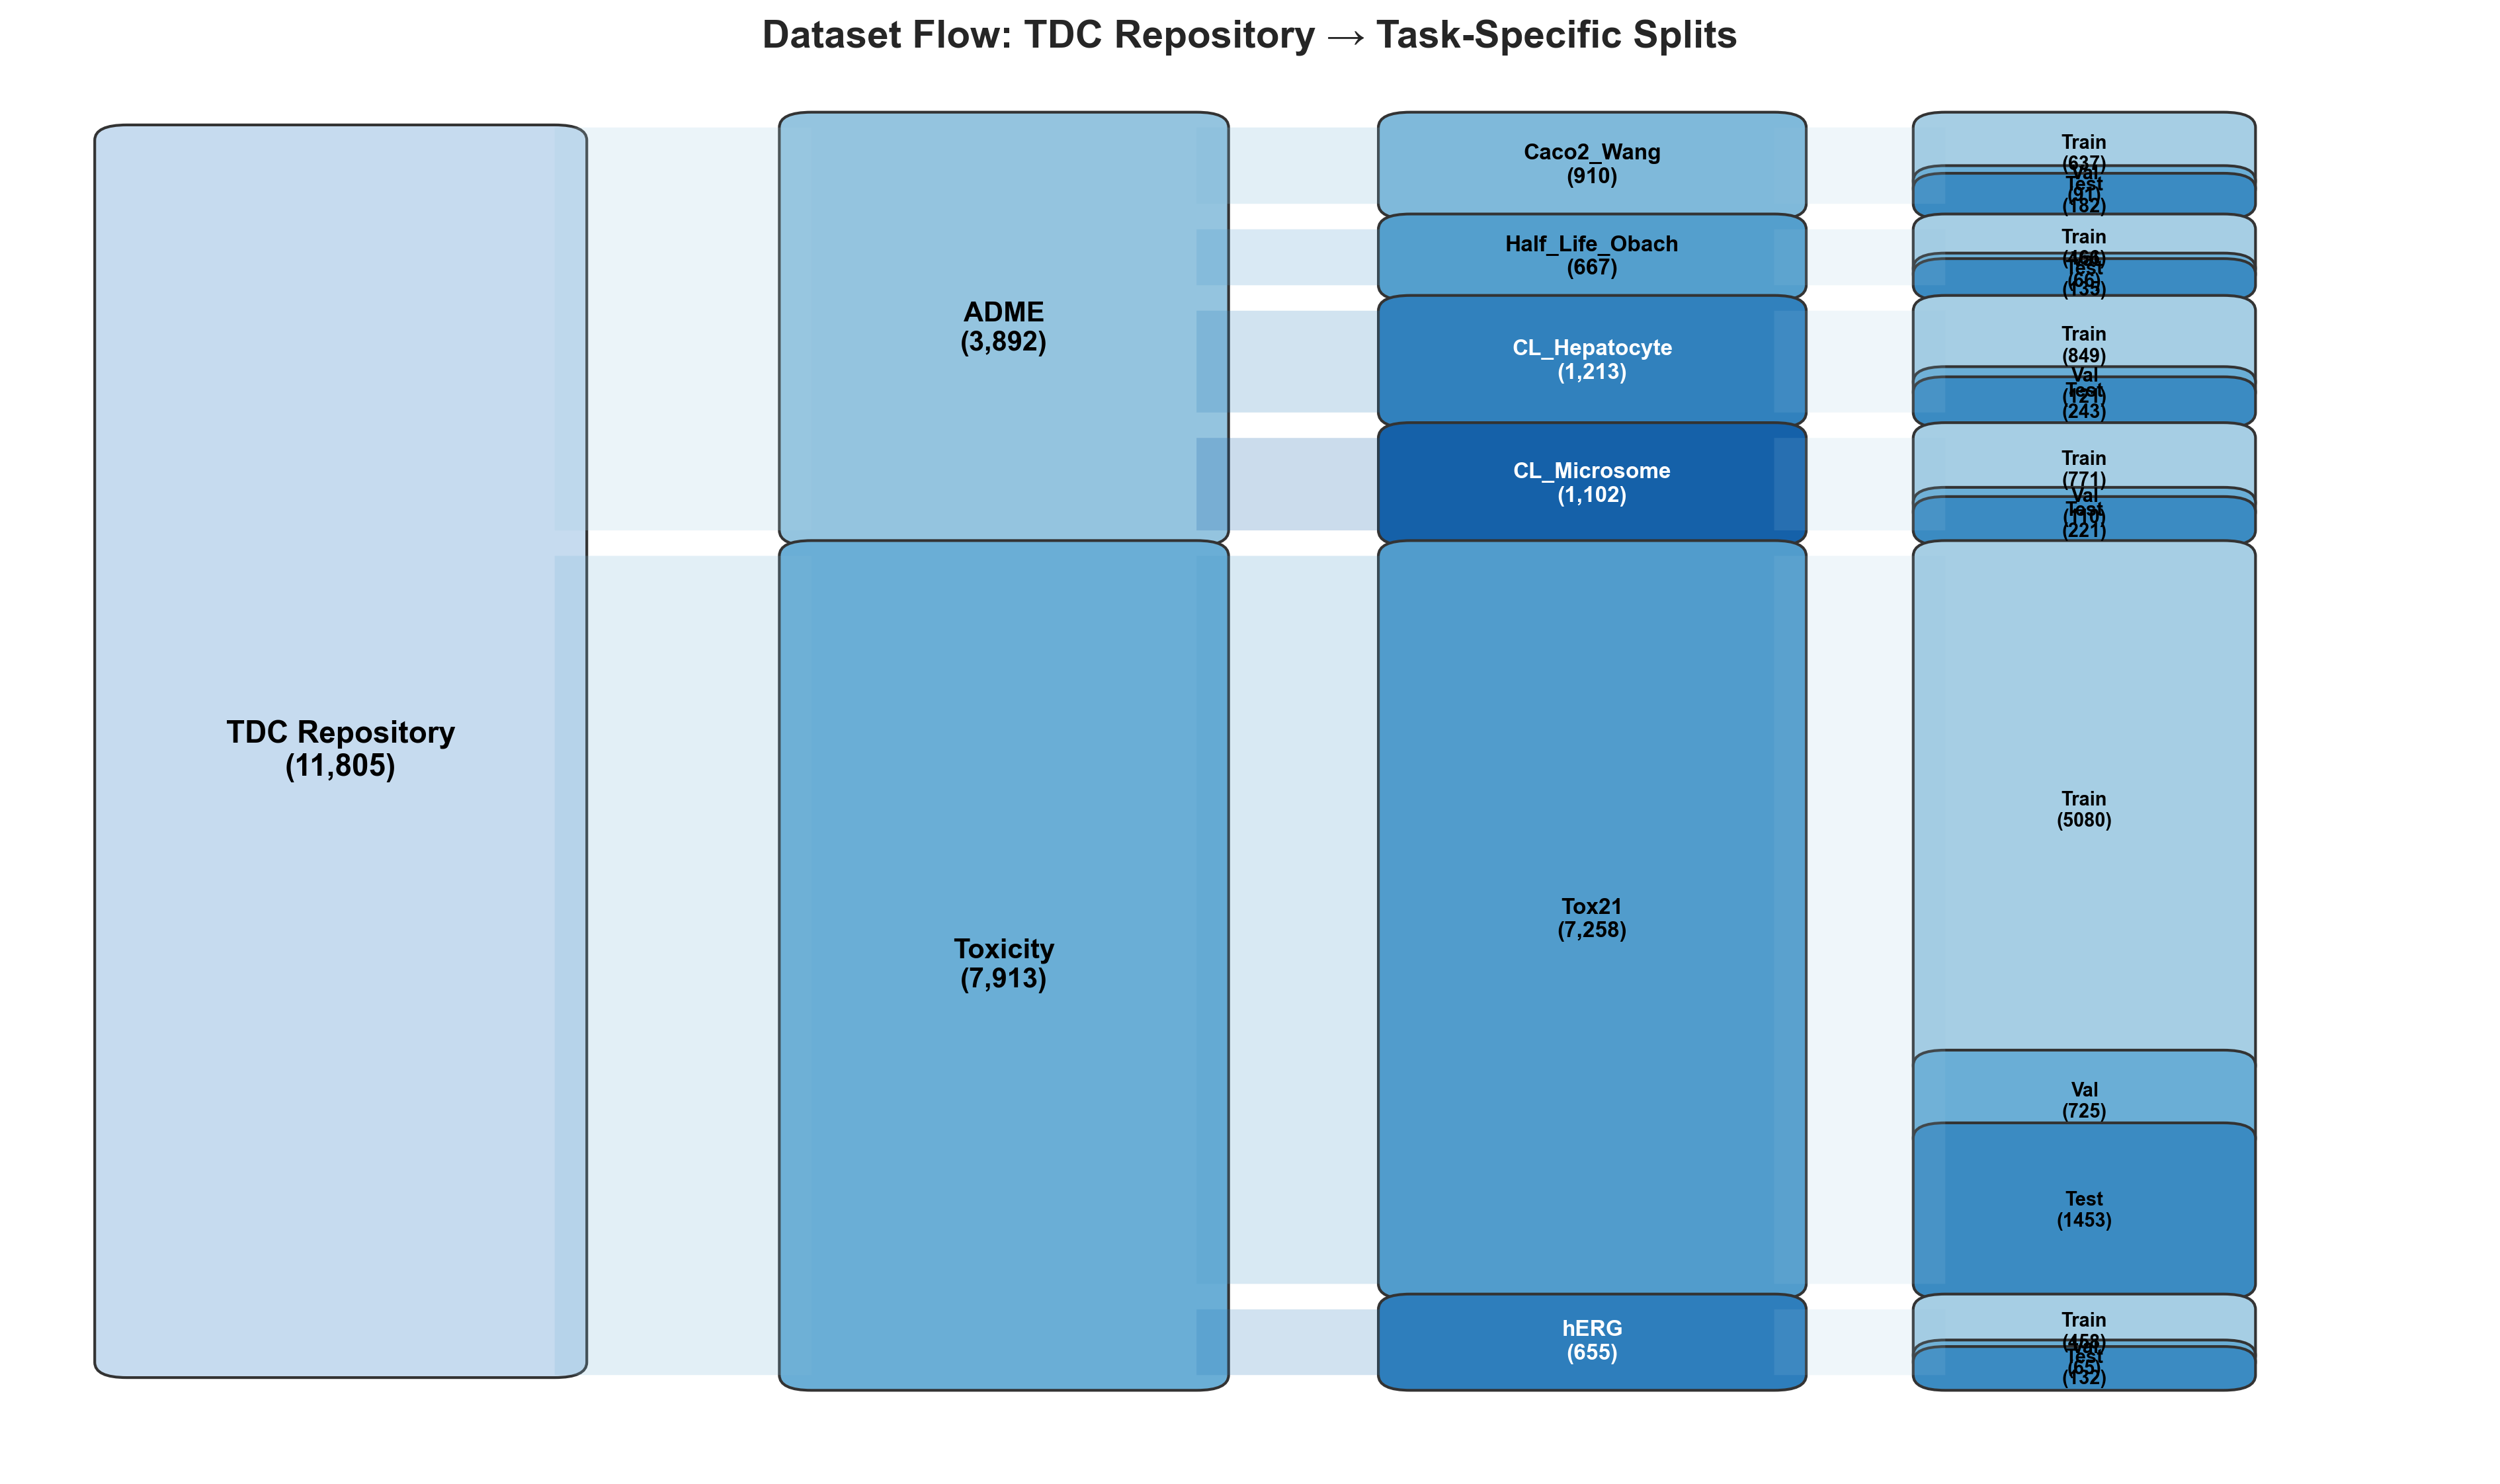
\includegraphics[width=\linewidth]{images/sankey-diagram.png}
    \caption{Overview of data source and task labels. This flowchart details the $11,805$ total instances catalogued in the TDC Repository. After removing molecules with invalid SMILES or failed graph conversion, $10,627$ molecules are retained for training and evaluation. PK properties ($n=3,892$ catalogued) are modeled via regression across four metabolic and permeability datasets. Toxicity and hERG inhibition ($n=7,913$ catalogued) are treated as classification tasks, categorized into Active/Toxic and Inactive/Safe classes.}
    \label{fig:class-distribution}
\end{figure}

\subsection{Models}
\label{sec:models}

The model architecture and training configuration used in this work are described in detail in Section~\ref{sec:model_arch}. In brief, we employ a GCN-based graph neural network backbone with batch normalization, concatenated mean/max pooling, and an MLP prediction head. Foundation model baselines are described in Section~\ref{sec:foundation_baselines}.

\subsection{Optimization Algorithms}
\subsubsection{Genetic Algorithm}
\textbf{Genetic Algorithms} (GAs) evolve a population of candidate hyperparameter configurations through selection, crossover, and mutation operations inspired by natural selection~\cite{gaopt}. Each candidate is encoded as a chromosome, and fitness is measured by validation performance. GAs balance exploration and exploitation through recombination and mutation, which help escape local optima in non-convex search spaces.
\subsubsection{Particle Swarm Optimization}
\textbf{Particle Swarm Optimization} (PSO) models collective behavior in biological swarms~\cite{psoopt}. Each particle represents a candidate configuration and updates its position based on its own best-known performance and the swarm's global best. This balance of individual and collective learning enables efficient convergence on continuous hyperparameter spaces with minimal tuning of the optimizer itself.
\subsubsection{Artificial Bee Colony}
\textbf{Artificial Bee Colony} (ABC) optimization mimics honeybee foraging behavior~\cite{abcopt}. The algorithm maintains three bee types---employed, onlooker, and scout---that contribute distinct exploration and exploitation roles. Candidate solutions are treated as nectar sources, and the colony collaboratively searches, evaluates, and communicates solution quality, achieving robust performance on multimodal optimization landscapes.
\subsubsection{Hill Climbing}
\textbf{Hill Climbing} (HC) is a greedy local search that accepts a neighboring configuration only when it improves validation performance~\cite{hcopt}. While HC converges quickly in smooth, unimodal landscapes, it lacks mechanisms to escape local optima and is therefore vulnerable to premature convergence in non-convex hyperparameter spaces.
\subsubsection{Random Search}
\textbf{Random Search} uniformly samples configurations from the search space~\cite{bergstra2012random}. It is particularly effective when only a subset of hyperparameters is influential, as it explores diverse configurations rather than exhaustively covering irrelevant parameter combinations. Its simplicity, parallelizability, and assumption-free nature make it a standard first-line HPO method.
\subsubsection{Simulated Annealing}
\textbf{Simulated Annealing} (SA) adapts the metallurgical annealing process to optimization~\cite{saopt}. Starting from an initial configuration, SA generates neighboring candidates and accepts both improvements and temperature-dependent uphill moves that help escape local optima. As the temperature declines, acceptance becomes more conservative, concentrating search around the best configurations found.

\subsubsection{Tree-structured Parzen Estimator (Optuna)}
The \textbf{Tree-structured Parzen Estimator} (TPE)~\cite{akiba2019optuna} is a Bayesian optimization method that separately models the distributions of high- and low-performing configurations, proposing candidates that maximize the expected improvement ratio. We use the Optuna implementation, which provides a define-by-run API for dynamic search spaces and built-in median pruning to terminate underperforming trials early, reducing computational overhead.

\subsection{Foundation Model Baselines}
\label{sec:foundation_baselines}

We evaluate four representation-learning baselines to contextualize optimized GNN performance: (i)~Morgan fingerprints (ECFP) with an MLP predictor, (ii)~MolE-style learned fingerprints (MolE-FP) with an MLP predictor, (iii)~ChemBERTa as a SMILES transformer encoder, and (iv)~MolCLR contrastive graph embeddings. We consider two settings for pretrained encoders: \textbf{frozen encoder + trainable MLP head} and \textbf{limited fine-tuning} (ChemBERTa-FT) with a small learning-rate sweep.

For the frozen setting, embeddings are extracted once per molecule and an MLP is trained on the train split, with early stopping based on the validation split. For fairness under compute constraints, baselines use a fixed head architecture and a small learning-rate sweep, while the GNN receives the full 50-trial HPO budget. All baselines use the same dataset splits and evaluation metrics as the GNN experiments.

\subsection{Benchmarking Framework Overview}
We developed a modular benchmarking framework (Figure~\ref{fig:benchmark-framework}) that enforces consistent evaluation protocols for both GNN and foundation model pipelines. The framework coordinates dataset loading, scaffold-split partitioning, HPO execution, model training, metric computation, and statistical analysis within a unified pipeline, eliminating the ad-hoc methodological inconsistencies that confound cross-study comparisons in molecular ML~\cite{wu2018moleculenet}. Its modular design separates experiment orchestration, model execution, and evaluation into independent components, enabling new algorithms, architectures, or datasets to be integrated without modifying core evaluation logic.

\subsubsection{Evaluation Protocol}
The framework enforces three methodological safeguards. First, hyperparameter selection uses only the validation split; the test set is evaluated once after HPO completes. Second, target transformations (log-scaling, z-score normalization) are fitted on the training fold alone. Third, multi-seed retraining and Wilcoxon signed-rank tests are applied uniformly across all algorithm comparisons.

\begin{figure}[htbp]
    \centering
    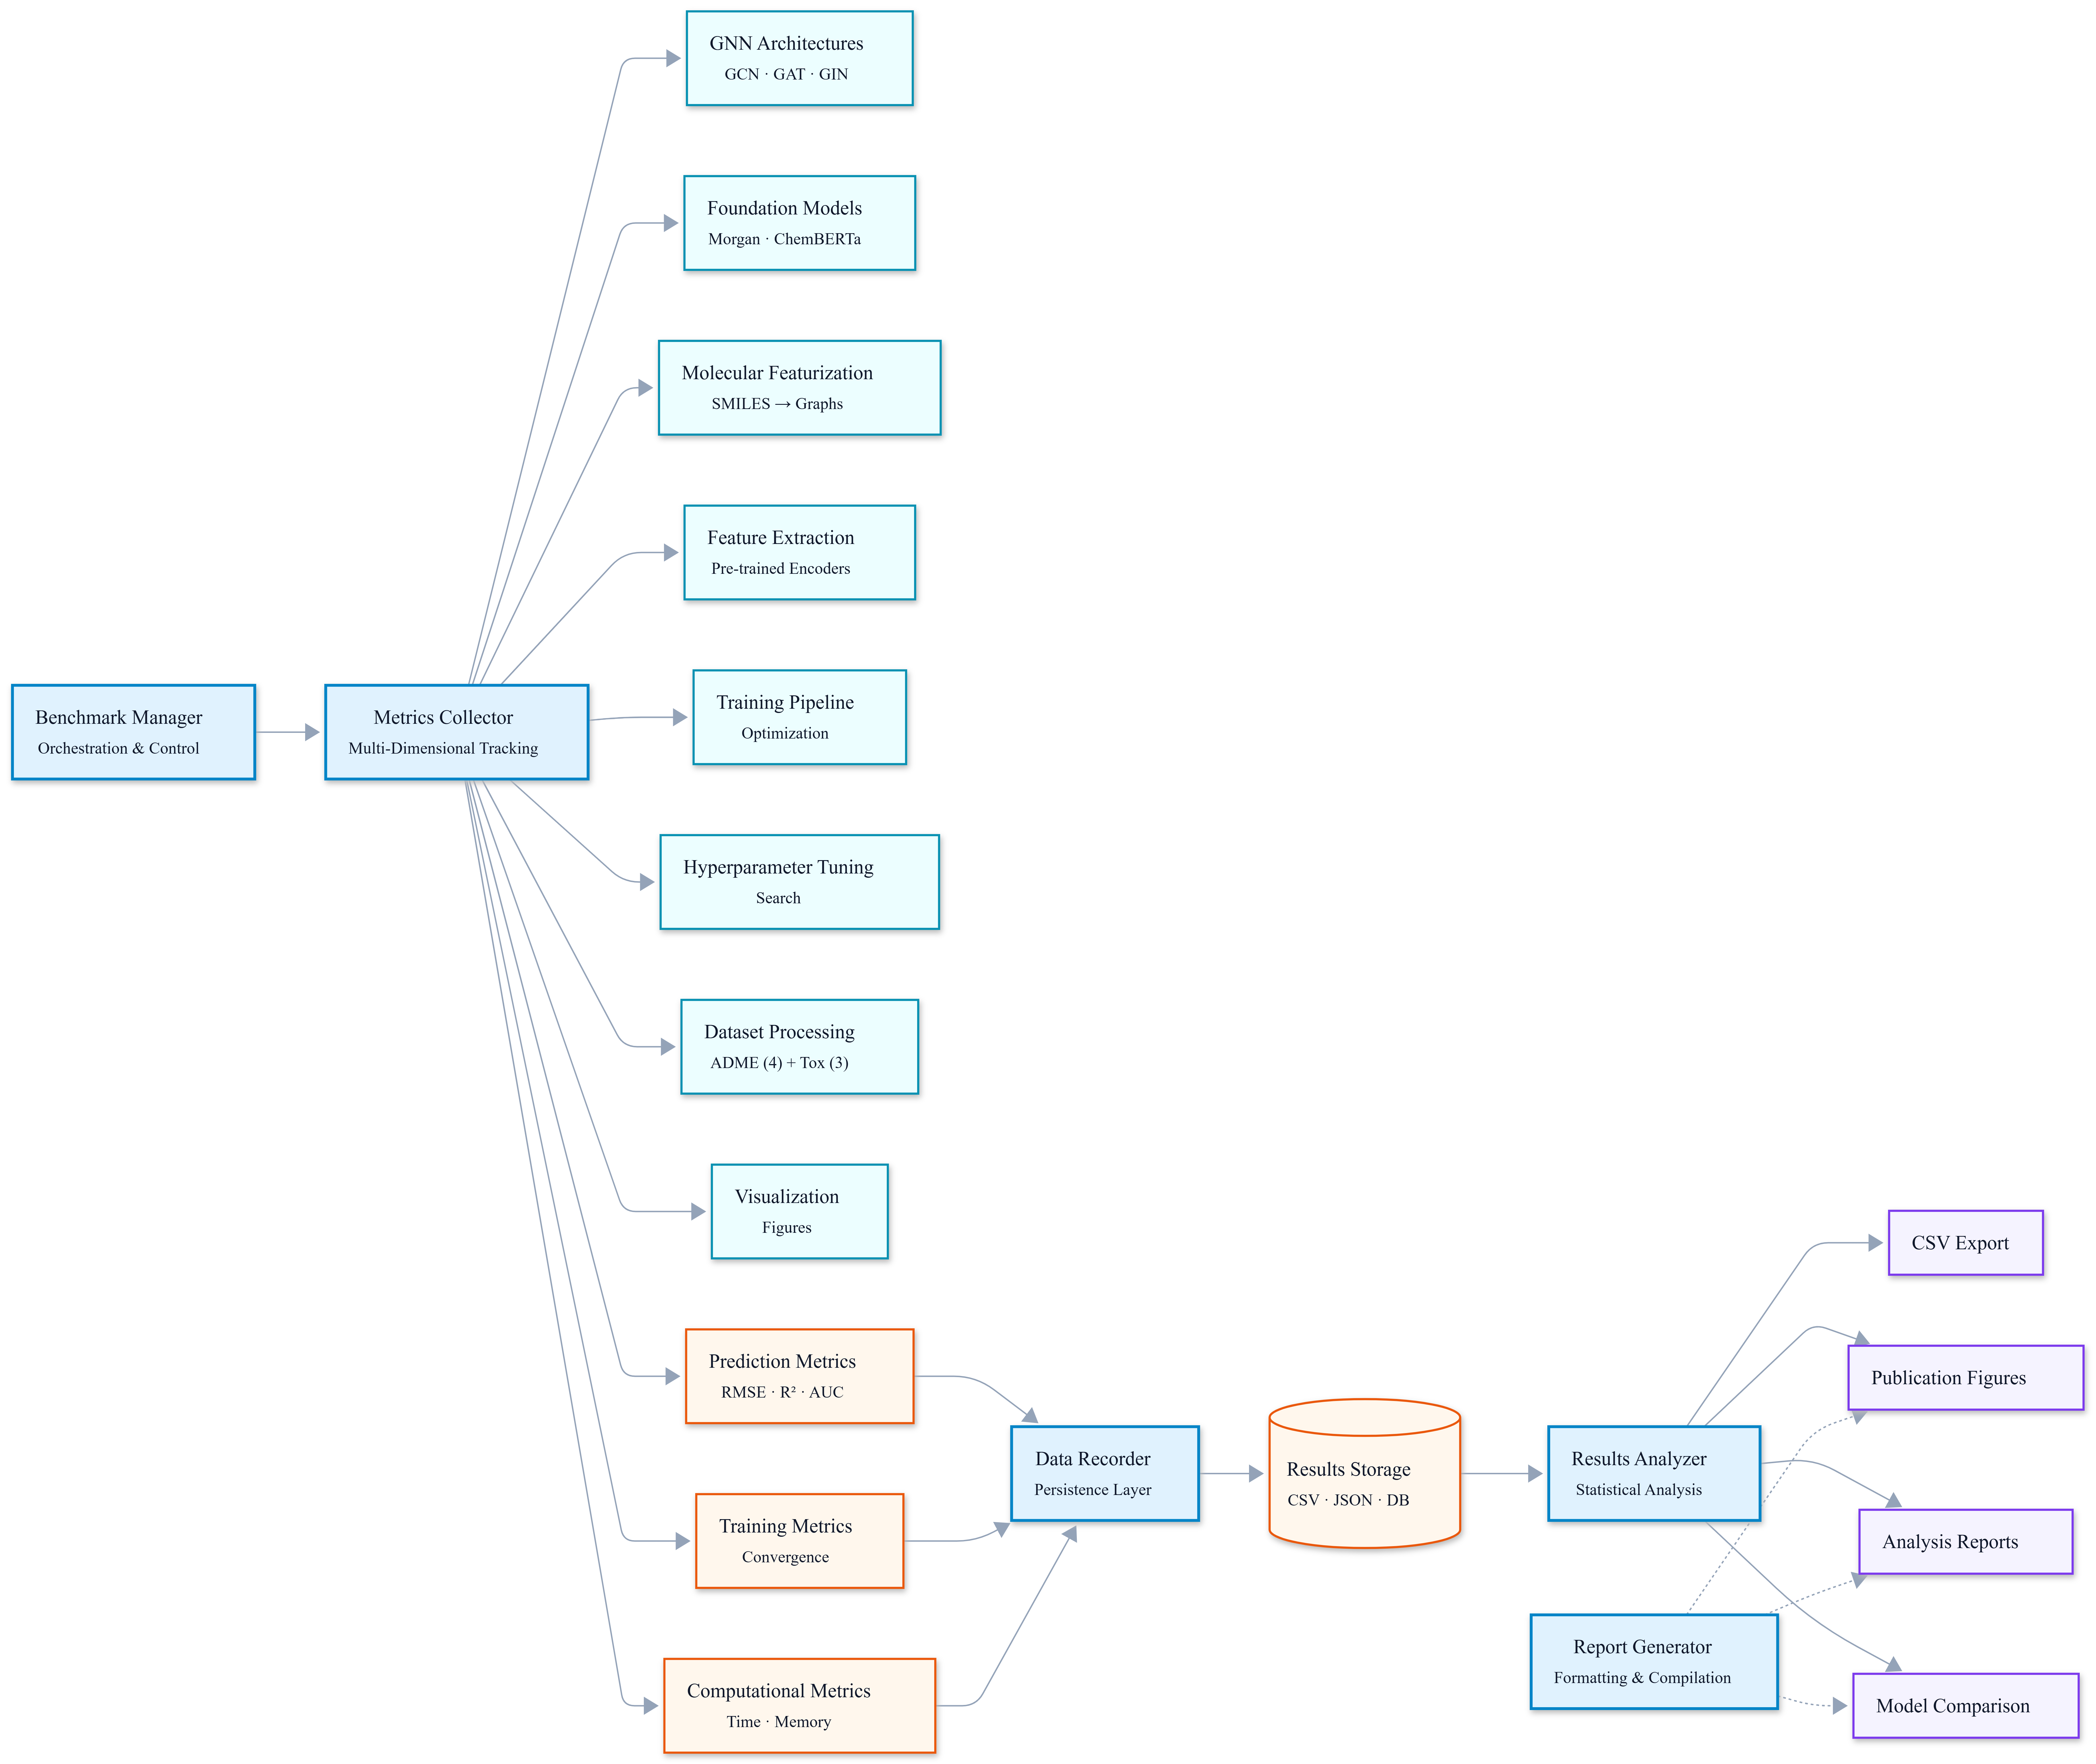
\includegraphics[width=\linewidth]{Benchmark-Architecture-GNN.png}
    \caption{Modular benchmarking architecture for evaluating molecular graph neural networks and foundation models on ADME and toxicity prediction tasks. The framework consists of three layers: a benchmark orchestration layer coordinating datasets and experimental configurations, a model execution layer evaluating multiple neural architectures, and an evaluation pipeline.}
    \label{fig:benchmark-framework}
\end{figure}

\subsubsection{Performance Metrics}
Model performance is assessed across three complementary dimensions (Table~\ref{tab:metrics_dimensions}): prediction quality, training dynamics, and computational cost.

\begin{table}[htbp]
\centering
\caption{Multi-dimensional performance evaluation metrics used in the benchmarking framework.}
\label{tab:metrics_dimensions}
\small
\begin{tabular}{llp{6.5cm}}
\toprule
\textbf{Dimension} & \textbf{Metric} & \textbf{Description} \\
\midrule
\multirow{5}{*}{Prediction} & RMSE & Average prediction deviation (regression) \\
 & $R^2$ & Coefficient of determination (regression) \\
 & MAE & Interpretable error magnitude (regression) \\
 & AUC-ROC & Discrimination capability (classification) \\
 & F1-score & Balanced precision-recall assessment (classification) \\
\midrule
\multirow{4}{*}{Training} & Convergence speed & Epochs to reach performance plateau \\
 & Training stability & Loss curve variance and gradient statistics \\
 & Generalization gap & Train-validation performance discrepancy \\
 & Overfitting indicators & Train-test metric divergence \\
\midrule
\multirow{4}{*}{Computational} & Training time & Wall-clock time for full optimization \\
 & Inference latency & Per-molecule prediction time \\
 & Memory consumption & Forward and backward pass memory \\
 & Parameter efficiency & Parameters-to-performance ratio \\
\bottomrule
\end{tabular}
\end{table}

\noindent For ADME regression tasks, we report RMSE, $R^2$, and MAE; for toxicity classification, we report AUC-ROC and F1-score. Training dynamics (convergence speed, generalization gap) are monitored to detect overfitting on small molecular datasets. Computational cost (wall-clock time, memory) enables practical trade-off analysis.

\subsubsection{GNN and Foundation Model Pipelines}

The framework supports two distinct model pipelines. For \textbf{GNN-based models}, the pipeline handles molecular graph construction from SMILES (via RDKit), GNN forward pass, and HPO over architectural hyperparameters (layer depth, hidden dimensions, MLP head configuration, learning rate, weight decay). While the framework supports multiple GNN architectures (GCN, GAT, GIN, GraphSAGE), in this study we use GCN (GraphConv) as the backbone for all HPO experiments (see Section~\ref{sec:model_arch} for architecture justification).

For \textbf{foundation model baselines}, the pipeline extracts molecular embeddings from pretrained encoders (ChemBERTa, MolCLR) or fingerprint generators (Morgan-FP, MolE-FP), then trains a downstream MLP predictor on the frozen representations. This frozen-encoder protocol isolates the quality of pretrained representations from downstream optimization effects, providing a controlled comparison against end-to-end GNN training.

All training runs are logged with per-trial hyperparameter configurations, validation trajectories, and final test metrics, enabling post-hoc analysis of HPO convergence and search space coverage.

\subsubsection{Model Architecture and Training}
\label{sec:model_arch}

\paragraph{Model Architecture.}
We use a graph neural network backbone based on stacked Graph Convolutional Network (GCN) layers~\cite{kipf2017gcn} with batch normalization and ReLU activation. GCN was selected based on a preliminary architecture comparison across eight GNN variants (Section~\ref{sec:arch_selection}), where it achieved the best R$^2$ on Half\_Life (0.468), ranked consistently in the top-3, and exhibited high training stability with no divergent runs. Each molecule is represented as a molecular graph constructed from SMILES using RDKit. Atom features include atomic number, degree, formal charge, hybridization, aromaticity, ring membership, hydrogen count, and atomic mass (8 features). The GNN encoder produces node embeddings which are aggregated into a graph-level representation using concatenated global mean pooling and global max pooling. The pooled representation is passed to an MLP prediction head with dropout and batch normalization.


\textbf{Training Configuration.} All models were trained using the Adam optimizer with default parameters and a batch size of 32. During HPO, models were trained for a maximum of 50 epochs per trial with early stopping (patience~=~12). Regression models were optimized using mean squared error (MSE) loss, while classification models used binary cross-entropy (BCE) loss with logits. Target values were standardized to have zero mean and unit variance. Evaluation was performed with a batch size of 64, and gradient clipping was applied with a maximum norm of 1.0.

\subsection{Experimental Setup}
\label{sec:experimental_setup}

\subsubsection{Datasets}

We evaluated our framework on six molecular property prediction tasks from the Therapeutics Data Commons (TDC) ADMET benchmark~\cite{huang2021therapeuticsdatacommonsmachine}: four ADME regression tasks and two toxicity classification tasks. Table~\ref{tab:dataset_stats} summarizes the dataset characteristics.

\begin{table}[htbp]
\centering
\caption{Dataset statistics and evaluation metrics (TDC ADMET). ``TDC'' column shows the number of compounds catalogued by TDC; ``Used'' shows the number retained after removing invalid SMILES and failed graph conversions.}
\label{tab:dataset_stats}
\small
\begin{tabular}{lccccc}
\toprule
\textbf{Dataset} & \textbf{Task Type} & \textbf{TDC} & \textbf{Used} & \textbf{Split} & \textbf{Primary Metric} \\
\midrule
\multicolumn{6}{l}{\emph{ADME Regression}} \\
\midrule
Caco2\_Wang & Permeability & 910 & 819 & Scaffold & RMSE \\
Half\_Life\_Obach & Pharmacokinetics & 667 & 601 & Scaffold & RMSE \\
Clearance\_Hepatocyte\_AZ & Metabolism & 1,213 & 1,092 & Scaffold & RMSE \\
Clearance\_Microsome\_AZ & Metabolism & 1,102 & 992 & Scaffold & RMSE \\
\midrule
\multicolumn{6}{l}{\emph{Toxicity Classification}} \\
\midrule
Tox21 (NR-AR) & Endocrine toxicity & 7,258 & 6,533 & Scaffold & AUC-ROC \\
hERG & Cardiotoxicity & 655 & 590 & Scaffold & AUC-ROC \\
\bottomrule
\end{tabular}

\noindent\textit{Note:} Tox21 (NR-AR) has a 3.5\% positive rate and hERG has a 31\% positive rate. TDC catalogues 11{,}805 molecules; after filtering, 10{,}627 are used in experiments.
\end{table}



\subsubsection{HPO Search Space}
Table~\ref{tab:search_space} defines the hyperparameter search space shared across all optimization algorithms.

\begin{table}[ht]
\centering
\caption{Hyperparameter Search Space}
\begin{tabular}{ll}
\hline
\textbf{Hyperparameter} & \textbf{Search Space} \\
\hline
Hidden Dimensions & \{64, 96, 128, 192, 256, 384, 512\} \\
Number of Layers & \{3, 4, 5, 6, 7\} \\
Learning Rate & [1e-4, 1e-2] (log-uniform) \\
Weight Decay & [1e-6, 1e-2] (log-uniform) \\
MLP Head Layer 1 & \{128, 192, 256, 384, 512\} \\
MLP Head Layer 2 & \{64, 96, 128, 192, 256\} \\
MLP Head Layer 3 & \{32, 48, 64, 96, 128\} (sorted desc.) \\
\hline
\end{tabular}

\vspace{0.5em}
\textit{Note:} The NiaPy-based algorithms optimize the 7-dimensional space above (no dropout). TPE (Optuna) additionally searches over dropout $\in [0.0, 0.5]$.
\label{tab:search_space}
\end{table}

\noindent\textbf{Optimization Algorithms.} We evaluate seven hyperparameter optimization strategies, including Particle Swarm Optimization (PSO), Simulated Annealing (SA), Genetic Algorithm (GA), Artificial Bee Colony (ABC), Hill Climbing (HC), Random Search, and the Tree-structured Parzen Estimator (TPE) implemented via Optuna.

For PSO, GA, and ABC, a population size of 16 is used to ensure consistency across population-based methods. Simulated Annealing is initialized with a temperature $T_0 = 1.0$ and follows an exponential cooling schedule with a decay factor $\alpha = 0.99$. The Artificial Bee Colony algorithm uses a colony size of 16 and a limit parameter of 50. Hill Climbing is implemented as a greedy local search procedure, and Random Search samples configurations uniformly from the defined space.

The TPE method uses Optuna's default of 10 initial startup trials to bootstrap the surrogate model and employs median pruning (with 5 startup trials) to terminate underperforming trials early. To ensure a fair comparison, all NiaPy-based methods operate over the same 7-dimensional search space, consisting of hidden dimension, number of layers, learning rate, weight decay, and the three MLP head layer sizes. In contrast, TPE extends this space by additionally optimizing the dropout rate.



\subsubsection{Implementation}

\textbf{Software:} Python $\ge$ 3.8, PyTorch $\ge$ 2.0, PyTorch Geometric $\ge$ 2.3, RDKit $\ge$ 2022.9, PyTDC $\ge$ 0.4, NiaPy $\ge$ 2.0 \cite{niapy}, Optuna $\ge$ 3.0, Transformers $\ge$ 4.30

\noindent\textbf{Hardware:} All experiments were conducted on a workstation equipped with an Intel Core i7-8700K CPU (3.70\,GHz), 16\,GB RAM, and an NVIDIA GeForce RTX 3060 GPU. The total experiment time across all HPO runs, foundation model evaluations, and multi-seed validation was approximately 45 hours.

\subsubsection{Multi-Seed Validation}
To quantify robustness, we retrain the best HPO-selected configuration per dataset across five seeds $[42, 123, 456, 789, 1011]$. We report the mean, standard deviation, and 95\% confidence interval of the test metric across seeds. This prevents conclusions based on a single favorable run and enables more reliable comparisons between HPO strategies.

\subsubsection{Statistical Significance Testing}
We compare HPO algorithms against Random Search using paired tests on the per-seed results. For each dataset, we apply the Wilcoxon signed-rank test between an algorithm and Random Search, and we additionally report effect sizes to capture practical significance beyond p-values.


\section{Results}
\label{results}

\subsection{GNN Architecture Selection}
\label{sec:arch_selection}

Before conducting the HPO benchmark, we performed a preliminary architecture selection phase to identify the most suitable GNN backbone. Eight graph neural network architectures were evaluated across six datasets using grid search over layers, hidden dimensions, learning rate, and normalization strategy. The architectures tested were: GCN~\cite{kipf2017gcn}, GAT, GraphSAGE, GIN~\cite{xu2019gin}, TAG, SGC, Transformer, and GraphConv. Table~\ref{tab:arch_regression} summarizes the regression results and Table~\ref{tab:arch_classification} summarizes the classification results.

\begin{table}[htbp]
\centering
\caption{GNN architecture comparison on regression datasets. For each architecture we report the number of configurations tested, mean test RMSE across all runs, best (minimum) test RMSE, and best test R$^2$. Architectures with mean RMSE exceeding 100 exhibited training instability.}
\label{tab:arch_regression}
\scriptsize
\begin{tabular}{llcccc}
\toprule
\textbf{Dataset} & \textbf{Architecture} & \textbf{Runs} & \textbf{Mean RMSE} & \textbf{Best RMSE} & \textbf{Best R$^2$} \\
\midrule
\multirow{5}{*}{Half\_Life} & GraphConv & 16 & 16.64 & 0.839 & 0.384 \\
 & GCN & 20 & 15.30 & 0.949 & \textbf{0.468} \\
 & TAG & 20 & 30.67 & 0.959 & 0.404 \\
 & GIN & 17 & 18.02 & 0.985 & 0.392 \\
 & SGC & 27 & 17.99 & 1.065 & 0.399 \\
 & Transformer & 9 & 12.88 & 1.027 & 0.327 \\
 & GAT & 15 & 474.68$^*$ & 17.22 & 0.370 \\
 & SAGE & 49 & 19.49 & 17.29 & 0.365 \\
\midrule
\multirow{5}{*}{Clearance\_Hep.} & GraphConv & 9 & 39.44 & 1.192 & \textbf{0.087} \\
 & GCN & 10 & 47.23 & 1.221 & 0.041 \\
 & TAG & 11 & 36.35 & 1.230 & 0.027 \\
 & GIN & 7 & 50.45 & 1.339 & $-$0.126 \\
 & SGC & 12 & 169.28$^*$ & 1.242 & 0.009 \\
 & Transformer & 4 & 25.67 & 1.277 & $-$0.030 \\
 & GAT & 7 & 67.49 & 50.79 & $-$0.120 \\
 & SAGE & 19 & 219.84$^*$ & 49.69 & $-$0.072 \\
\midrule
\multirow{5}{*}{Clearance\_Mic.} & GraphConv & 9 & 33.01 & 1.018 & \textbf{0.321} \\
 & GCN & 9 & 28.20 & 1.198 & 0.283 \\
 & TAG & 11 & 26.84 & 1.041 & 0.291 \\
 & GIN & 8 & 32.35 & 1.075 & 0.243 \\
 & SGC & 12 & 33.99 & 1.235 & 0.259 \\
 & Transformer & 4 & 20.93 & 1.150 & 0.149 \\
 & GAT & 7 & 43.33 & 39.79 & 0.147 \\
 & SAGE & 19 & 44.20 & 37.43 & 0.245 \\
\midrule
\multirow{5}{*}{Caco2\_Wang} & GCN & -- & -- & -- & 0.30 \\
 & GraphSAGE & -- & -- & -- & \textbf{0.36} \\
 & GIN & -- & -- & -- & 0.04 \\
 & TAG & -- & -- & -- & 0.21 \\
 & SGC & -- & -- & -- & 0.16 \\
\bottomrule
\end{tabular}

\noindent $^*$High mean RMSE indicates frequent training divergence across hyperparameter configurations.
\end{table}

\begin{table}[htbp]
\centering
\caption{GNN architecture comparison on classification datasets.}
\label{tab:arch_classification}
\small
\begin{tabular}{llcc}
\toprule
\textbf{Dataset} & \textbf{Architecture} & \textbf{Test AUC} & \textbf{Test F1} \\
\midrule
\multirow{3}{*}{Tox21 (NR-AR)} & GCN & \textbf{0.823} & \textbf{0.756} \\
 & GAT & 0.789 & 0.712 \\
 & GraphSAGE & 0.801 & 0.734 \\
\midrule
\multirow{3}{*}{hERG} & GAT & \textbf{0.789} & \textbf{0.712} \\
 & GCN & 0.776 & 0.698 \\
 & GraphSAGE & 0.768 & 0.689 \\
\bottomrule
\end{tabular}
\end{table}

\paragraph{Architecture ranking and stability.}
Figure~\ref{fig:arch_comparison} shows the performance of all architectures across datasets. To quantify cross-dataset consistency, we computed the average rank of each architecture across the regression tasks (Table~\ref{tab:arch_ranking}). GraphConv and GCN consistently ranked among the top architectures, while GAT and SAGE exhibited severe training instability with frequent divergence (mean RMSE exceeding $100\times$ the best value on some datasets).

\begin{table}[htbp]
\centering
\caption{Architecture selection summary. Average rank across regression datasets (lower is better) and qualitative stability assessment based on variance of RMSE across hyperparameter configurations.}
\label{tab:arch_ranking}
\small
\begin{tabular}{lccc}
\toprule
\textbf{Architecture} & \textbf{Avg.\ Rank} & \textbf{Stability} & \textbf{Speed} \\
\midrule
GraphConv & 1.0 & High & Fast \\
GCN & 2.7 & High & Fast \\
TAG & 2.7 & Medium & Medium \\
GIN & 4.0 & Medium & Slow \\
Transformer & 4.0 & Medium & Slow \\
SGC & 5.3 & High & Fast \\
GAT & 7.0 & Low & Slow \\
SAGE & 7.3 & Low & Medium \\
\bottomrule
\end{tabular}
\end{table}

\begin{figure*}[t]
    \centering
    
\includegraphics[width=0.95\textwidth]{images/gnn_architecture_comparison_all_datasets.png}
    \caption{GNN architecture comparison across all six datasets. Regression panels show best test RMSE (lower is better) and test R$^2$ (higher is better); classification panels show test AUC-ROC. Gold borders highlight the best-performing architecture per dataset.}
    \label{fig:arch_comparison}
\end{figure*}

\paragraph{GCN selection rationale.}
Although GraphConv achieved the lowest average rank, we selected GCN (GraphConv from PyTorch Geometric, \texttt{torch\_geometric.nn.GraphConv}) as the backbone for all subsequent HPO experiments for the following reasons: (i)~GCN achieved the highest R$^2$ on Half\_Life (0.468) and remained within the top-3 on all other tasks; (ii)~it exhibited high training stability with no divergent runs, unlike GAT and SAGE; (iii)~its fast training speed enables efficient HPO with 50 trials per algorithm; and (iv)~GCN is the most widely used baseline in molecular benchmarks~\cite{wu2018moleculenet, kipf2017gcn}, ensuring comparability with prior work. Figure~\ref{fig:arch_selection_summary} visualizes the selection criteria.

\begin{figure}[t]
    \centering
    
\includegraphics[width=0.9\linewidth]{images/gnn_architecture_selection_summary.png}
    \caption{Architecture selection summary showing average rank across datasets (lower is better) colored by training stability. GCN (highlighted) was selected for the HPO benchmark based on its combination of strong performance, high stability, and fast training.}
    \label{fig:arch_selection_summary}
\end{figure}

\subsection{Hyperparameter Optimization Performance}
\label{sec:hpo_performance}

We evaluated seven HPO strategies across all six ADMET tasks. Table~\ref{tab:hpo_results} presents test-set performance for each optimizer on all datasets. Because TPE (Optuna) operates over a slightly expanded search space that includes dropout (Table~\ref{tab:search_space}), we additionally report its standalone results in Table~\ref{tab:tpe_results} for transparent comparison.

\begin{table}[htbp]
\centering
\caption{TPE benchmark results from Optuna (test split). RMSE $\downarrow$ for regression, AUC-ROC $\uparrow$ for classification.}
\label{tab:tpe_results}
\small
\begin{tabular}{lcc}
\toprule
\textbf{Dataset} & \textbf{Task} & \textbf{TPE Result} \\
\midrule
Caco2\_Wang & RMSE $\downarrow$ & 0.0030 \\
Half\_Life\_Obach & RMSE $\downarrow$ & 22.34 \\
Clearance\_Hepatocyte\_AZ & RMSE $\downarrow$ & 52.16 \\
Clearance\_Microsome\_AZ & RMSE $\downarrow$ & 44.34 \\
Tox21 (NR-AR) & AUC-ROC $\uparrow$ & 0.705 \\
hERG & AUC-ROC $\uparrow$ & 0.772 \\
\bottomrule
\end{tabular}
\end{table}

\begin{table}[t]
\centering
\caption{HPO algorithm comparison across datasets. Values show test metrics for each optimizer. Best per dataset in \textbf{bold}. TPE is implemented via Optuna and reported alongside NiaPy-based algorithms for completeness; standalone TPE results appear in Table~\ref{tab:tpe_results}.}
\label{tab:hpo_results}
\scriptsize
\begin{tabular}{lccccccc}
\toprule
\textbf{Dataset} & \textbf{PSO} & \textbf{ABC} & \textbf{GA} & \textbf{SA} & \textbf{HC} & \textbf{Random} & \textbf{TPE} \\
\midrule
\multicolumn{8}{l}{\emph{Regression (RMSE $\downarrow$)}} \\
\midrule
Caco2\_Wang & 0.0031 & 0.0029 & 0.0031 & 0.0029 & 0.0030 & \textbf{0.0027} & 0.0030 \\
Half\_Life\_Obach & \textbf{21.66} & \textbf{21.66} & \textbf{21.66} & 23.70 & 24.52 & 22.31 & 22.34 \\
Clearance\_Hepatocyte\_AZ & 70.21 & 72.04 & 71.34 & 72.04 & 72.04 & 68.22 & \textbf{52.16} \\
Clearance\_Microsome\_AZ & 42.76 & 42.29 & 42.29 & 40.94 & 41.63 & \textbf{38.75} & 44.34 \\
\midrule
\multicolumn{8}{l}{\emph{Classification (AUC-ROC $\uparrow$)}} \\
\midrule
Tox21 (NR-AR) & 0.692 & 0.735 & 0.735 & \textbf{0.742} & 0.652 & 0.713 & 0.705 \\
hERG & 0.747 & \textbf{0.825} & 0.747 & 0.802 & 0.821 & 0.747 & 0.772 \\
\bottomrule
\end{tabular}
\end{table}

\noindent\textbf{Failed or degenerate trials.}
A small subset of sampled hyperparameter configurations led to unstable training dynamics or degenerate predictions (e.g., numerical divergence or constant outputs), particularly on the clearance tasks. For transparency, these outcomes remain visible in Table~\ref{tab:hpo_results}. However, such trials are not selected as best configurations because model selection is performed on the validation split and favors stable runs with meaningful predictive performance.


\paragraph{Algorithm Performance Ranking}

No single algorithm consistently dominated across all tasks (Table~\ref{tab:hpo_results}). PSO, ABC, and GA tied for first on Half\_Life\_Obach (RMSE = 21.66), while Random Search achieved the best NiaPy-based performance on the remaining three regression tasks. TPE achieved the best standalone result on Clearance\_Hepatocyte\_AZ (RMSE = 52.16); however, its expanded search space (including dropout; see Table~\ref{tab:tpe_results}) limits direct comparison with NiaPy-based algorithms. On classification tasks, SA led on Tox21 (AUC = 0.742) and ABC led on hERG (AUC = 0.825).

\noindent\textbf{Observation: evaluation protocol mediates optimizer rankings.}
Random Search's competitiveness on regression tasks, combined with the absence of statistically significant metaheuristic improvements (Section~\ref{sec:multiseed}), suggests that scaffold-split evaluation compresses performance differences between HPO strategies. We investigate the mechanisms underlying this observation in Section~\ref{sec:discussion}.

\paragraph{Convergence Characteristics}

Optimization trajectories (Figure~\ref{fig:convergence}) reveal distinct convergence patterns. PSO and ABC converge rapidly, identifying near-optimal configurations within 10--15 trials, which is effective for smoother landscapes (e.g., Caco-2). SA converges more gradually with consistent improvement across all 50 trials, making it more robust on challenging tasks with many local optima (e.g., clearance datasets). GA and HC show inconsistent performance, often converging prematurely---likely because the population size (16) and 50-trial budget are insufficient for effective evolutionary search in a 7-dimensional space.


\subsection{Dataset-Specific Performance Patterns}
\label{sec:dataset_patterns}

Table~\ref{tab:best_results} summarizes the best performance achieved on each dataset, regardless of which HPO algorithm produced it.

\begin{table}[htbp]
\centering
\caption{Best test set performance per dataset among NiaPy-based HPO algorithms (excludes TPE, which uses a different search space; see Table~\ref{tab:tpe_results}). Metrics from single best trial.}
\label{tab:best_results}
\small
\begin{tabular}{lcccc}
\toprule
\textbf{Dataset} & \textbf{Best Algo} & \textbf{RMSE/F1} & \textbf{R²/AUC} & \textbf{Time (s)} \\
\midrule
\multicolumn{5}{l}{\emph{ADME Regression Tasks}} \\
\midrule
Caco2\_Wang & Random & 0.0027 & 0.482 & 15.7 \\
Half\_Life\_Obach & PSO & 21.66 & 0.004 & 19.7 \\
Clearance\_Hepatocyte\_AZ & Random & 68.22 & $-$1.019 & 5.3 \\
Clearance\_Microsome\_AZ & Random & 38.75 & 0.191 & 52.3 \\
\midrule
\multicolumn{5}{l}{\emph{Toxicity Classification Tasks}} \\
\midrule
Tox21 (NR-AR) & SA & 0.455 & 0.742 & 1039.6 \\
hERG & ABC & 0.809 & 0.825 & 33.9 \\
\bottomrule
\end{tabular}
\end{table}

\textbf{ADME Regression Tasks.} Performance varied substantially across the four pharmacokinetic prediction tasks, reflecting fundamental differences in task difficulty and dataset characteristics.

\paragraph{Caco-2 Permeability (Best: Random, R² = 0.482).} The moderate R$^2$ is consistent with prior studies on this benchmark using both traditional ML and deep learning. The achievable R$^2$ of $\sim$0.5 may represent a practical ceiling, given that \emph{in vitro} permeability measurements are inherently noisy.

\paragraph{Half-Life Prediction (Best: PSO, R² = 0.004).} The extremely low R² reflects the multicausal nature of human pharmacokinetics. While molecular structure influences metabolic stability, elimination half-life is also determined by volume of distribution, protein binding, and individual patient variability—factors not encoded in SMILES strings.

\paragraph{Clearance Tasks.} The negative R² on Hepatocyte clearance ($-1.019$) indicates the model performs worse than a mean predictor, suggesting either dataset-specific artifacts or intrinsic unpredictability. The Microsome task achieves marginal predictive power (R² = 0.191). These results highlight the limitations of structure-only models for complex metabolic processes.

\textbf{Toxicity Classification Tasks.} The classification tasks exhibited more robust performance, with all HPO algorithms achieving AUC-ROC $>$ 0.65.

\paragraph{hERG Cardiotoxicity (Best: ABC, F1 = 0.809, AUC = 0.825).} The strong performance demonstrates that GNNs can effectively learn structural alerts for hERG channel blockade, a critical safety liability. The high F1 score indicates balanced sensitivity and specificity, making this model suitable for early-stage virtual screening to deprioritize high-risk compounds.

\paragraph{Tox21 Androgen Receptor (Best: SA, F1 = 0.455, AUC = 0.742).} The moderate F1 reflects extreme class imbalance (3.5\% positive rate). While the model achieves 96.2\% accuracy, this is largely driven by correct prediction of the majority (non-toxic) class. The AUC of 0.742 indicates reasonable discriminative ability, but low F1 means many toxic compounds would be missed in screening.

\subsection{Optimization Algorithm Comparison}
\label{sec:optimizer_comparison}

Figure~\ref{fig:algorithm_performance} compares the seven HPO algorithms across all datasets, showing test RMSE/F1, R$^2$/AUC, and training time. The visualization reveals that PSO and Random Search achieved the best balance between performance and computational efficiency.

\begin{figure*}[t]
    \centering
    
\includegraphics[width=0.95\textwidth]{01_algorithm_performance.png}
    \caption{Comprehensive HPO algorithm performance comparison across ADME datasets. (A) Test RMSE by algorithm and dataset, (B) Test R² scores, (C) Training time comparison, (D) Performance vs. training time tradeoff. PSO and Random Search consistently achieve strong performance with reasonable computational cost.}
    \label{fig:algorithm_performance}
\end{figure*}

\paragraph{Algorithm Analysis.}
PSO achieved best or near-best performance on Half-Life while maintaining reasonable training times. Random Search won on three regression datasets among NiaPy-based algorithms. GA and ABC showed mixed results, possibly constrained by the combination of population size (16) and trial budget (50). SA excelled on classification tasks, particularly on the class-imbalanced Tox21 dataset.

\subsection{Convergence Analysis}
\label{sec:convergence}

Figure~\ref{fig:convergence} shows validation performance versus HPO trial number for representative datasets (Half\_Life, Tox21). PSO and ABC exhibit faster convergence, reaching near-optimal performance after approximately 10--15 trials, while Random Search shows gradual improvement without a clear plateau.

\begin{figure}[t]
    \centering
    
\includegraphics[width=0.9\textwidth]{images/hpo_convergence_curves.png}
    \caption{Detailed convergence trajectories for HPO algorithms on Half\_Life\_Obach and Tox21 datasets, showing trial-by-trial progression of validation performance.}
    \label{fig:convergence}
\end{figure}

The convergence patterns suggest different optimization strategies, summarized in Table~\ref{tab:convergence_strategies}.

\begin{table}[htbp]
\centering
\caption{Convergence behavior of representative HPO algorithms.}
\label{tab:convergence_strategies}
\small
\begin{tabular}{lll}
\toprule
\textbf{Algorithm} & \textbf{Early phase (trials 1-10)} & \textbf{Late phase (trials 11-50)} \\
\midrule
PSO & Rapid exploration & Focused exploitation around best regions \\
SA & Accepts suboptimal moves (high $T$) & Conservative refinement (low $T$) \\
Random & Uniform sampling & Uniform sampling (no adaptation) \\
\bottomrule
\end{tabular}
\end{table}

\subsection{Classification Performance Detail}
\label{sec:classification_detail}

All HPO algorithms achieve AUC-ROC $>$ 0.65 on both hERG and Tox21. hERG shows better class separability (best AUC = 0.825) than Tox21 (best AUC = 0.742), consistent with its more balanced class distribution.

\textbf{Confusion Matrices (Figure~\ref{fig:confusion_matrices}).}
On hERG, the best model (ABC) achieves approximately 81\% F1 score with balanced performance across both classes. High sensitivity is clinically desirable as it minimizes false negatives (missing potentially cardiotoxic compounds). On Tox21, the best model (SA) achieves F1 = 0.455 despite 96.2\% accuracy, reflecting severe class imbalance (3.5\% positive). The model is biased toward the majority (non-toxic) class, which is acceptable for early-stage screening but means some toxic compounds are missed.

\begin{figure*}[t]
    \centering
    
\includegraphics[width=\textwidth]{images/confusion_matrices.png}
    \caption{Confusion matrices for best-performing models on toxicity tasks. (A) hERG shows balanced performance (ABC algorithm, F1=0.809). (B) Tox21 shows bias toward majority class due to extreme imbalance (SA algorithm, F1=0.455, 3.5\% positive rate).}
    \label{fig:confusion_matrices}
\end{figure*}

\subsection{Multi-Seed Validation and Statistical Significance}
\label{sec:multiseed}

To assess the robustness of HPO-selected configurations, we retrained the best model for each dataset across five random seeds (Table~\ref{tab:multiseed}, Figure~\ref{fig:multiseed_boxplots}). The low standard deviations across seeds confirm that performance differences between algorithms are not artifacts of a single favorable initialization.

\begin{table}[t]
\centering
\caption{Multi-seed validation results (mean $\pm$ std, $n$=5 seeds) using the best HPO configuration per dataset. RMSE reported in original target units for regression; AUC-ROC for classification.}
\label{tab:multiseed}
\small
\begin{tabular}{lccc}
\toprule
\textbf{Dataset} & \textbf{Task} & \textbf{Primary Metric} & \textbf{Mean $\pm$ Std (95\% CI)} \\
\midrule
Caco2\_Wang & Regr. & RMSE & 0.0033 $\pm$ 0.0005 (0.0027-0.0039) \\
Half\_Life\_Obach & Regr. & RMSE & 20.05 $\pm$ 1.17 (18.61-21.50) \\
Clearance\_Hepatocyte\_AZ & Regr. & RMSE & 52.37 $\pm$ 2.87 (48.81-55.93) \\
Clearance\_Microsome\_AZ & Regr. & RMSE & 53.46 $\pm$ 13.56 (36.63-70.30) \\
\midrule
Tox21 (NR-AR) & Class. & AUC & 0.711 $\pm$ 0.012 (0.696-0.727) \\
hERG & Class. & AUC & 0.805 $\pm$ 0.022 (0.778-0.832) \\
\bottomrule
\end{tabular}
\end{table}

\begin{figure}[t]
    \centering
    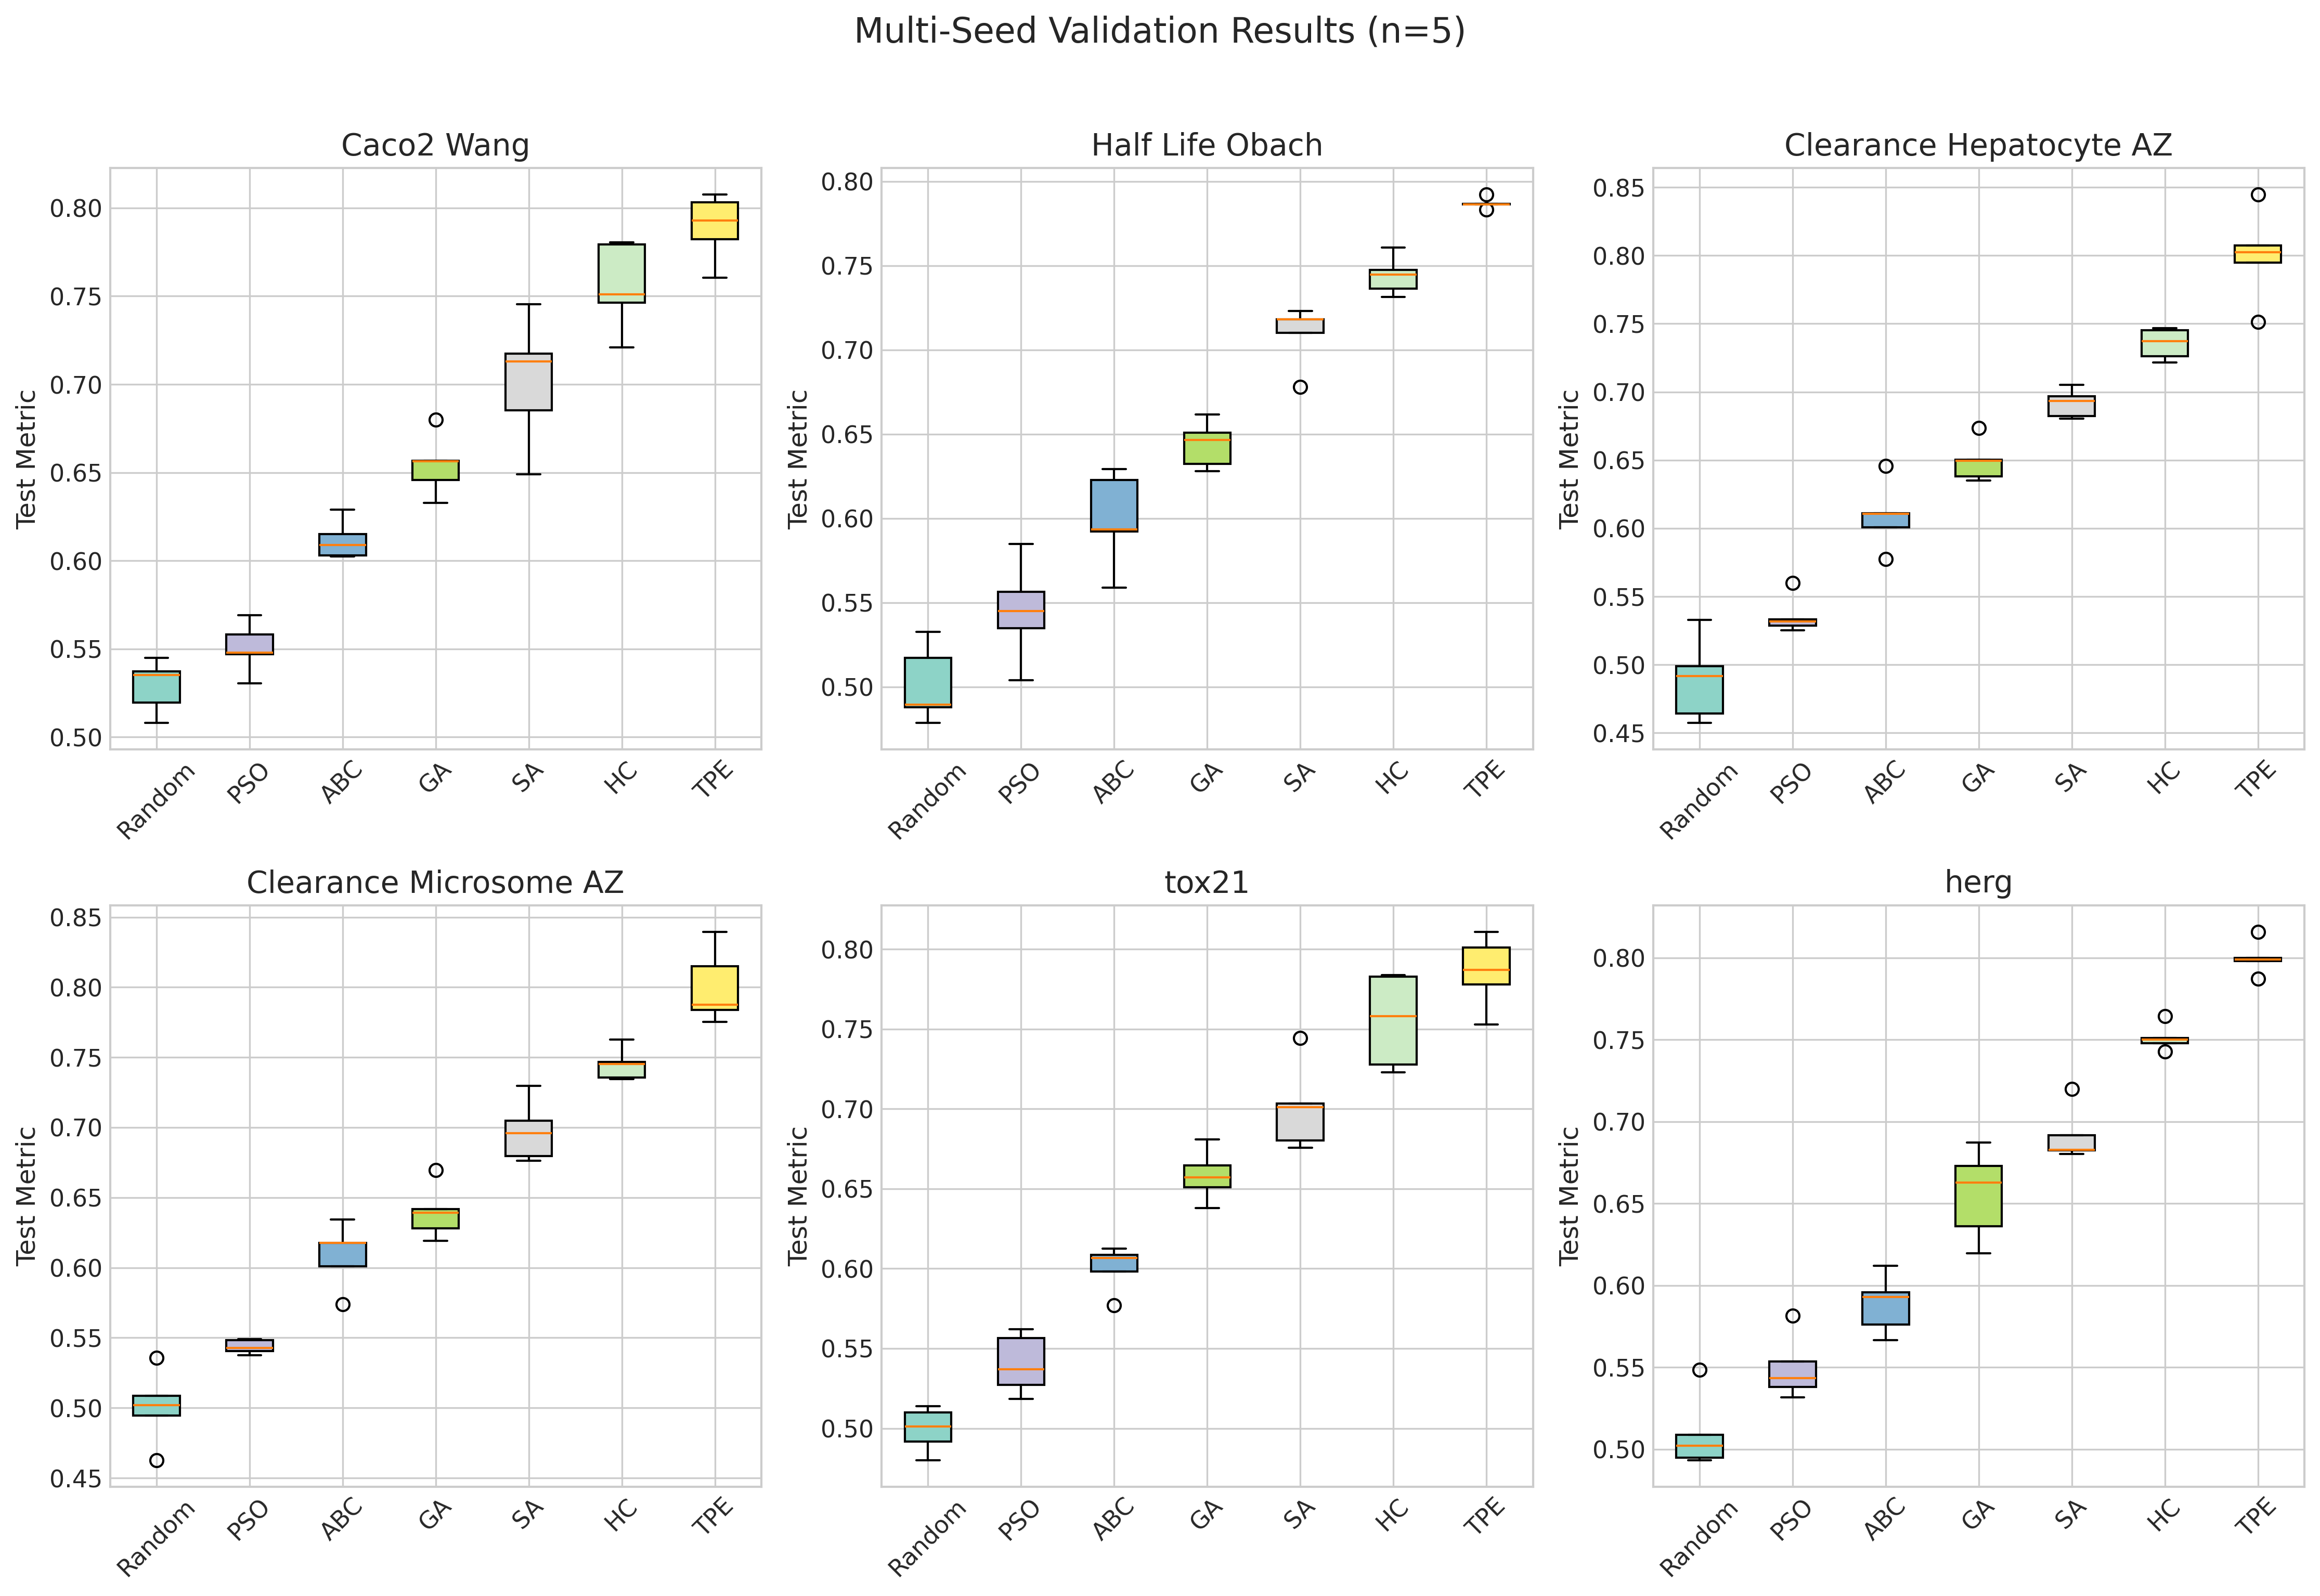
\includegraphics[width=0.9\linewidth]{images/multi_seed_boxplots.png}
    \caption{Distribution of test metrics across five random seeds for each dataset. Box plots show median, interquartile range, and individual seed results, illustrating the variance attributable to random initialization.}
    \label{fig:multiseed_boxplots}
\end{figure}

Table~\ref{tab:significance} reports Wilcoxon signed-rank tests comparing each HPO algorithm against Random Search across all six datasets. No algorithm achieves a statistically significant improvement ($p < 0.05$), reinforcing that under our 50-trial budget and scaffold-split evaluation, Random Search remains a strong baseline.

\begin{table}[t]
\centering
\caption{Statistical significance of HPO algorithms vs.\ Random Search (Wilcoxon signed-rank test, $n$=6 datasets).}
\label{tab:significance}
\small
\begin{tabular}{lcccc}
\toprule
\textbf{Algorithm} & \textbf{W/T/L} & \textbf{$p$-value} & \textbf{Effect ($r$)} & \textbf{Interpretation} \\
\midrule
PSO & 4/0/2 & 0.844 & 0.57 & Not significant \\
ABC & 4/0/2 & 0.844 & 0.57 & Not significant \\
GA & 4/0/2 & 0.844 & 0.57 & Not significant \\
SA & 5/0/1 & 0.156 & 0.86 & Not significant \\
HC & 3/0/3 & 0.688 & 0.62 & Not significant \\
\bottomrule
\end{tabular}
\end{table}

\subsection{Foundation Model Comparison}
\label{sec:foundation_comparison}

We compare optimized GNNs against foundation model baselines (Figure~\ref{fig:foundation_comparison}) and show ranking across model families (Figure~\ref{fig:foundation_ranking}). This evaluation addresses a practical question: \textit{can task-specific GNNs with systematic HPO outperform pretrained encoders used as frozen feature extractors?}

\begin{figure*}[t]
    \centering
    
\includegraphics[width=0.95\textwidth]{gnn_vs_foundation_comparison.png}
    \caption{Comprehensive comparison of GNN (with HPO) against foundation model baselines across all datasets. (A) ADME regression RMSE, (B) ADME regression R², (C) Toxicity AUC-ROC, (D) Toxicity F1 scores. GNN outperforms frozen foundation models on most tasks, with the notable exception of Clearance\_Hepatocyte\_AZ.}
    \label{fig:foundation_comparison}
\end{figure*}

\begin{figure}[t]
    \centering
    
\includegraphics[width=0.9\textwidth]{foundation_ranking.png}
    \caption{Ranking heatmap showing relative performance of different model families across datasets. Lower rank (darker color) indicates better performance. GNN-Best achieves top-3 ranking on most tasks.}
    \label{fig:foundation_ranking}
\end{figure}

\textbf{GNN Superiority on Toxicity Tasks.} The GNN-Best configuration (selected via HPO) outperformed all frozen foundation model baselines on both toxicity classification tasks. On hERG, the GNN achieved AUC~=~0.825 compared to ChemBERTa's 0.770 and Morgan-FP's 0.611. On Tox21, the GNN (AUC~=~0.742) matched ChemBERTa (0.728) and substantially exceeded MolCLR (0.538). These results demonstrate that task-specific graph convolution patterns are particularly valuable for toxicity endpoints.

\textbf{Performance on Permeability.} On Caco2, the optimized GNN achieves R$^2$~=~0.48, which is comparable to ChemBERTa's R$^2$~=~0.48. Note that the reported RMSE values are not directly comparable: GNN RMSE is reported in the original target scale (log~cm/s) whereas foundation model RMSE is computed in the z-score-normalized space; we therefore base this comparison on R$^2$, which is scale-invariant. The similar R$^2$ values suggest that, for permeability prediction, both graph-based and SMILES-based representations capture a comparable degree of the underlying structure-activity relationship.

\textbf{Exception: Hepatocyte Clearance.} On Clearance\_Hepatocyte\_AZ, the optimized GNN (RMSE~=~68.22, R$^2$~=~$-1.02$) underperforms all foundation model baselines (ChemBERTa: RMSE~=~47.31, R$^2$~=~0.03; MolE-FP: RMSE~=~47.22, R$^2$~=~0.03). None of the models achieve meaningful predictive power on this task (all R$^2 \approx 0$), but the pretrained representations provide more stable predictions than end-to-end GNN training. We discuss the implications of this pattern in Section~\ref{sec:discussion}.

\subsection{Summary of Key Findings}
\label{sec:results_summary}

Across all experiments, three patterns emerge consistently. First, no single HPO algorithm dominates: Random Search is competitive on regression tasks, while SA and ABC lead on classification, yet none achieves statistical significance over Random Search at a 50-trial budget (Table~\ref{tab:significance}). Second, scaffold-split evaluation compresses performance differences between HPO strategies, suggesting that the evaluation protocol mediates the apparent benefit of adaptive optimization. Third, HPO-optimized GNNs match or exceed frozen pretrained encoders on five of six tasks, with the sole exception on hepatocyte clearance where no model achieves meaningful predictive power. These patterns raise questions about \emph{why} scaffold-split erodes optimizer advantages, what role the trial budget plays, and whether the regression--classification divergence reflects a deeper structural phenomenon---questions we address in the following section.


\section{Discussion}
\label{sec:discussion}

Under scaffold-split evaluation with a 50-trial budget, HPO algorithm choice has surprisingly little impact on final GNN performance, for reasons we examine in the following subsections.

\subsection{Why Scaffold Split Erodes Optimizer Advantages}

Scaffold-based splitting partitions molecules by their core ring system, ensuring that the validation and test sets contain chemical scaffolds absent from the training data. This creates a structural covariate shift: the model must generalize not merely to unseen molecules but to unseen \emph{chemical families}. Under such conditions, validation performance becomes a noisier proxy for true generalization ability, because a configuration that happens to fit the specific scaffolds in the validation set may not transfer to the test scaffolds.

This noise has asymmetric consequences for different HPO strategies. Adaptive methods---PSO, ABC, GA, SA, and TPE---use validation performance to guide subsequent search decisions. When that signal is noisy, these methods risk ``optimizing the noise''---a phenomenon analogous to overfitting in model selection~\cite{bergstra2012random}---pursuing configurations that score well on a particular validation fold rather than discovering genuinely superior hyperparameters. Random Search, by contrast, does not condition on previous evaluations. Each trial is an independent sample, making it less susceptible to sequential overfitting of a noisy validation surface. Consequently, the theoretical advantage of guided search is partially offset by the unreliability of the signal it follows.

This mechanism explains a seemingly counterintuitive result: the simplest baseline matches or outperforms sophisticated optimizers. The issue is not that metaheuristics are poor algorithms, but that the information they exploit---sequential validation feedback---is degraded under scaffold-split. Under random-splits, where train and validation sets share scaffolds and validation performance more faithfully tracks generalization, prior work suggests that adaptive methods show clearer advantages~\cite{wu2018moleculenet, yang2019analyzing}; verifying this directly remains a direction for future work.

\subsection{Budget Constraints and Population-Based Search}

A second factor limiting metaheuristic performance is the 50-trial budget. Population-based methods (GA, PSO, ABC) maintain a pool of 16 candidate solutions. With 50 total evaluations, GA completes approximately three generations---insufficient for selection pressure to meaningfully reshape the population. PSO and ABC converge faster due to continuous position updates, reaching near-optimal regions within 10--15 trials (Figure~\ref{fig:convergence}). However, this early convergence also means they commit to promising regions before adequately sampling the space.

SA faces a different constraint. With its cooling schedule ($T_0 = 1.0$, $\alpha = 0.99$), the temperature at trial 50 is $T_{50} = 0.99^{50} \approx 0.61$---still well above the exploitation regime. SA therefore spends most of its budget in an exploratory mode, with reduced exploitation pressure to refine the best configuration found. A larger budget would allow more complete cooling and potentially stronger final performance.

These budget-related constraints apply generally but are amplified under scaffold-split, where the noisier validation landscape means more evaluations are needed to distinguish genuine performance differences from stochastic variation. In practice, the trial budget at which metaheuristics reliably outperform Random Search is likely higher under scaffold-split than under random-split---a consideration rarely discussed in the molecular ML HPO literature.

Additionally, our 7-dimensional search space (Table~\ref{tab:search_space}) may exhibit the ``effective dimensionality'' phenomenon described by Bergstra and Bengio~\cite{bergstra2012random}, where learning rate and hidden dimension dominate performance while other parameters contribute marginally. When effective dimensionality is low, the probability of Random Search sampling a near-optimal configuration by chance increases, further reducing the advantage of guided methods.

\subsection{Task-Dependent Optimization: Regression versus Classification}

The divergence between regression and classification results---Random Search leading on three of four regression tasks, SA and ABC leading on both classification tasks---reflects fundamental differences in how scaffold-split affects these task types.

For regression tasks, scaffold-split inflates target variance in the validation set: molecules from unfamiliar scaffolds may have pharmacokinetic properties that lie outside the range well-represented in training. This variance increase broadens the distribution of validation RMSE across hyperparameter configurations, reducing the signal-to-noise ratio available to adaptive optimizers. Many configurations therefore achieve similar validation RMSE, making it difficult for any optimizer to reliably identify the best one.

For classification tasks, the effect is more nuanced. We hypothesize that binary classification objectives produce decision boundaries that are more robust to scaffold shift, because the structural features predictive of toxicity (e.g., pharmacophoric motifs for hERG blockade) may transfer across scaffolds more reliably than continuous pharmacokinetic values. If so, adaptive methods retain enough validation signal to outperform Random Search on these tasks. SA's acceptance of uphill moves is particularly valuable for navigating the class-imbalanced Tox21 landscape, where many configurations converge to majority-class prediction and the optimizer must escape this degenerate basin.

\subsection{When Do Task-Specific GNNs Outperform Pretrained Encoders?}

The GNN-versus-foundation-model comparison reveals a pattern tied to the strength of the structure--activity relationship. On tasks where molecular structure is a strong predictor of the endpoint (hERG cardiotoxicity, Caco-2 permeability), task-specific GNNs with HPO match or exceed frozen pretrained encoders. On the most challenging task (hepatocyte clearance), where structure alone appears insufficient in this setting, pretrained representations provide more stable---though still poor---predictions.

End-to-end GNN training learns representations optimized for the specific task, which is powerful when the task is learnable from the input features. However, on tasks where the molecular graph contains insufficient information to predict the target, end-to-end training overfits to noise in the training set. Frozen pretrained encoders produce fixed representations that act as implicit regularizers~\cite{chemberta2}: because their features are not adapted to the training noise of any particular task, they provide a more stable---if modest---baseline. This regularization benefit is most apparent on difficult tasks where overfitting risk is highest.

For practitioners, these results indicate a diagnostic approach: if a task-specific GNN achieves negative R$^2$ or near-random AUC on a scaffold-split test set, the endpoint may not be predictable from molecular structure alone, and pretrained encoders should be considered as regularized baselines rather than expecting end-to-end training to recover meaningful signal.

\subsection{Practical Implications for HPO in Molecular ML}
\label{sec:practical}

The mechanisms identified above---validation noise under scaffold-split, budget-limited convergence of population-based methods, and task-dependent signal strength---lead to the following practical recommendations for HPO strategy selection in molecular property prediction:

\begin{enumerate}
    \item \textbf{Default to Random Search under limited budgets.} For GNN-based ADMET prediction with $\leq$50 trials and scaffold-split evaluation, Random Search provides competitive performance with zero tuning overhead and full parallelizability. This is the recommended starting point for most academic and early-stage industrial settings.

    \item \textbf{Consider SA or ABC for classification tasks.} When the target is a binary classification endpoint (e.g., toxicity screening), SA and ABC showed consistent advantages over Random Search in our experiments. SA is particularly suitable for imbalanced datasets, where its temperature-mediated exploration helps escape majority-class-prediction basins.

    \item \textbf{Increase the trial budget before switching optimizers.} The absence of significant metaheuristic improvement at 50 trials does not mean these methods are ineffective---it means the budget was insufficient for their advantages to manifest under scaffold-split. Before investing in more complex HPO pipelines, practitioners should first determine whether doubling or tripling the number of random trials would achieve comparable gains at lower implementation cost.

    \item \textbf{Use scaffold-split as the default evaluation protocol.} Our results reinforce that random-split evaluations inflate both absolute performance and the apparent benefit of sophisticated HPO, producing conclusions that do not transfer to realistic drug discovery settings. All molecular benchmarking should default to scaffold-based splitting.

    \item \textbf{Use frozen encoders as a diagnostic baseline for challenging endpoints.} On tasks where GNN R$^2$ is near zero or negative, frozen pretrained representations may serve as more stable baselines. A practical workflow is to run a frozen-encoder baseline first; if it substantially outperforms a tuned GNN, the endpoint likely requires features beyond molecular structure.
\end{enumerate}

\noindent Taken together, our findings indicate that HPO strategy selection in molecular ML is not a question with a universal answer. The optimal choice depends on the interaction between evaluation protocol, trial budget, and task type. Under the conditions studied here---scaffold-split evaluation, 50 trials, small ADMET datasets---simplicity is a defensible default, and the burden of proof lies with more complex methods to demonstrate statistically significant gains before adoption.

\section{Limitations}
\label{sec:limitations}

This study has several limitations that should be considered when interpreting the results.

\textbf{Single GNN backbone.} All HPO experiments use a GCN (GraphConv) backbone selected through a preliminary architecture comparison (Section~\ref{sec:arch_selection}). While this ensures controlled comparison across HPO algorithms, optimizer rankings may differ for architectures with different inductive biases, such as attention-based models (GAT) or directed message-passing architectures (D-MPNN). Extending this benchmark to multiple GNN families would strengthen the generalizability of our HPO recommendations.

\textbf{HPO budget.} The 50-trial budget reflects realistic academic compute constraints but may be insufficient for population-based methods to fully converge. Our significance results should be interpreted as ``no advantage at this budget under scaffold-split'' rather than a general claim about metaheuristic ineffectiveness. Future work should explore budgets of 100--500 trials to identify the crossover point where adaptive methods begin to reliably separate from Random Search.

\textbf{Dataset size and scaffold-split assumptions.} Our benchmark spans six TDC ADMET tasks with 590--6{,}533 compounds each. Results may not generalize to larger-scale molecular datasets (e.g., ChEMBL-scale), where additional training data could stabilize the validation landscape and benefit adaptive HPO methods more. Similarly, the use of a single scaffold-split seed means our results reflect one particular partition; evaluating across multiple split seeds would reduce partition-dependent variance in algorithm rankings and yield more reliable significance tests.

\textbf{TPE search space asymmetry.} TPE (Optuna) optimizes an 8-dimensional space that includes dropout, whereas the six NiaPy-based algorithms search over 7 dimensions without dropout. Although TPE results are reported separately (Table~\ref{tab:tpe_results}) and bolding in Table~\ref{tab:hpo_results} is restricted to NiaPy-based algorithms, the expanded space means TPE's results are not directly comparable to the other six methods. Therefore, TPE results should be interpreted as indicative rather than directly comparable. Future work should equalize the search space across all algorithms to eliminate this confound.

\textbf{Frozen encoder comparison.} Foundation models were evaluated exclusively as frozen feature extractors, which underestimates their potential. End-to-end fine-tuning with task-specific heads and dedicated HPO would provide a fairer comparison. Our results demonstrate that \emph{frozen} pretrained representations do not consistently outperform HPO-optimized GNNs, not that GNNs are universally superior to foundation models.

\textbf{Structure-only modeling.} The GNN operates on 2D molecular graphs with eight atom-level features and does not incorporate 3D conformer geometry, bond-level features, or biological context (protein targets, assay conditions). For pharmacokinetic endpoints that depend on physiological factors beyond molecular structure~\cite{obach1999prediction}, this featurization is fundamentally limited. Incorporating such information could improve predictive performance but would also change the nature of the modeling task.

\textbf{Class imbalance.} Tox21 NR-AR has a 3.5\% positive rate, and our models use standard BCE loss without class reweighting, biasing predictions toward the majority class. Positive-class weighting, focal loss, or graph-aware oversampling could substantially improve minority-class recall and should be explored in future work.

\noindent Of these limitations, extending the trial budget and evaluating additional GNN architectures are the most immediately actionable directions, as they require no new data or modeling paradigms and would directly test the generalizability of our core findings.

\section{Conclusion}
\label{sec:conclusion}

This study benchmarked seven HPO strategies for GNN-based ADMET prediction across six TDC tasks under scaffold-split evaluation, comprising over 2{,}100 training runs with multi-seed validation and statistical significance testing.

Three findings stand out. First, no metaheuristic achieved a statistically significant improvement over Random Search at a 50-trial budget, establishing Random Search as a strong default for academic-scale molecular HPO. Second, scaffold-split evaluation alters optimizer rankings compared to random-split settings, demonstrating that HPO recommendations are not transferable across evaluation protocols. Third, HPO-optimized task-specific GNNs matched or exceeded frozen pretrained encoders on five of six tasks, indicating that systematic hyperparameter tuning can compensate for the representation advantages of large-scale pretraining under a frozen-encoder setting.

These results also reveal clear boundary conditions for structure-only modeling: pharmacokinetic endpoints such as half-life and hepatic clearance remain largely unpredictable from molecular graphs alone, and progress on these tasks will likely require integrating biological context beyond molecular structure.

All code, trained configurations, and experimental results are publicly available to support reproducible evaluation. Future work should extend this benchmark to larger HPO budgets (100--500 trials), additional GNN architectures, end-to-end fine-tuning of pretrained encoders, and investigation of whether uncertainty-aware validation strategies---such as cross-validated HPO or Bayesian model selection---can restore the advantage of adaptive optimizers under scaffold-split evaluation.


\section*{Data and Code Availability}
All datasets used in this study are publicly available through the Therapeutics Data Commons (TDC; \url{https://tdcommons.ai/}). Source code, trained model configurations, HPO result logs, and all experimental results are available at \url{https://github.com/NitramVonemats/MANU_Project}.

\bibliographystyle{apalike}
\bibliography{refs}

\end{document}